\documentclass[10pt,aspectratio=169,handout]{beamer}
\usetheme{Madrid}
\usecolortheme{whale}

\setbeamertemplate{navigation symbols}{}
\setbeamertemplate{footline}[frame number]

\usepackage[utf8]{inputenc}
\usepackage[T1]{fontenc}
\usepackage[italian]{babel}
\usepackage{amsmath,amssymb,mathtools}
\usepackage{graphicx}
\usepackage{booktabs}
\usepackage{algorithm}
\usepackage{algpseudocode}
\usepackage{xcolor}
\usepackage{hyperref}

% --- Colori Sapienza ---
\definecolor{sapienzared}{HTML}{802433}
\definecolor{sapienzagold}{RGB}{193,154,80}

% --- Colori Beamer ---
\setbeamercolor{frametitle}{fg=white,bg=sapienzared}
\setbeamercolor{title}{fg=white,bg=sapienzared}
\setbeamercolor{structure}{fg=sapienzared}

\setbeamercolor{palette primary}{fg=white,bg=sapienzared}
\setbeamercolor{palette secondary}{fg=white,bg=sapienzared}
\setbeamercolor{palette tertiary}{fg=white,bg=sapienzared}
\setbeamercolor{palette quaternary}{fg=white,bg=sapienzared}

% --- Colori aggiuntivi per i block ---
\definecolor{blockbluegray}{HTML}{2F3E46}
\definecolor{sapienzagoldsoft}{HTML}{C19A50}

% --- Block normali ---
\setbeamercolor{block title}{fg=white,bg=blockbluegray}
\setbeamercolor{block body}{fg=black,bg=gray!7}

% --- Alert block: oro Sapienza ---
\definecolor{sapienzagoldsoft}{HTML}{C19A50}

\setbeamercolor{block title alerted}{fg=black,bg=sapienzagoldsoft}
\setbeamercolor{block body alerted}{fg=black,bg=yellow!8}

\title[Randomized SVD]{Randomized Singular Value Decomposition}
\subtitle{Teoria e Applicazioni: compressione immagini e Reduced Order Modeling}
\author{Michele Magrini \and Francesco Massimi \and Gianluca Marino}
\institute{Data Mining - Matematica Applicata}
\date{}

\titlegraphic{
    \vspace{-0.4cm}
    
\includegraphics[width=5cm]{Uniroma1.svg.png}
}

\begin{document}

% 1
\begin{frame}
  \titlepage
\end{frame}

% 2
\begin{frame}{Introduzione}
\begin{itemize}
  \item Molti dataset e modelli numerici ad alta dimensione hanno una struttura \textbf{intrinsecamente low-rank}.
  \item La SVD fornisce la migliore approssimazione di rango $k$, ma diventa costosa per matrici grandi.
  \item La \textbf{Randomized SVD} usa proiezioni casuali per stimare il sottospazio dominante con costo inferiore.
  \item Obiettivo del progetto: confrontare SVD e rSVD su:
  \begin{itemize}
    \item compressione di immagini;
    \item POD e POD-DEIM per PDE non lineari.
  \end{itemize}
\end{itemize}
\vspace{0.2cm}
\begin{block}{Idea chiave}
Approssimare bene le direzioni dominanti senza decomporre direttamente tutta la matrice.
\end{block}
\end{frame}

% 3
\begin{frame}{Singular Value Decomposition (SVD)}
Sia $A\in\mathbb{R}^{m\times n}$ con rango $r$. La SVD è
\[
A = U\Sigma V^T,
\]
dove $U \in \mathbb{R}^{m\times m}$ e $V \in \mathbb{R}^{n\times n}$ sono ortogonali e $\Sigma \in \text{diag}_{m\times n}$ contiene i valori singolari
\[
\sigma_1\geq\sigma_2\geq\cdots\geq\sigma_r>0.
\]
\pause
L'approssimazione troncata di rango $k$ è
$A_k = U_k\Sigma_k V_k^T.$
\begin{block}{Teorema di Eckart--Young--Mirsky}
$A_k$ è la migliore approssimazione di rango $k$ in norma spettrale e Frobenius:
\[
\|A-A_k\|_2=\sigma_{k+1}, \qquad
\|A-A_k\|_F^2=\sum_{j=k+1}^{r}\sigma_j^2.
\]
\end{block}
\end{frame}

% 4
\begin{frame}{Randomized Singular Value Decomposition (rSVD)}
\begin{columns}[T]
\column{0.52\textwidth}
\begin{enumerate}
  \item Genera una matrice casuale gaussiana:
  \[
  \Omega\in\mathbb{R}^{n\times(k+p)}.
  \]
  \item Campiona il range dominante:
  \[
  Y=A\Omega \in \mathbb{R}^{m\times(k+p)}.
  \]
  \item Ortonormalizza: $Y=QR,$
  \[
  Q \in \mathbb{R}^{m \times (k+p)} \ \ \text{ortogonale},
  \]
  \[
  R\in \mathbb{R}^{(k+p)\times(k+p)} \ \ \text{triangolare superiore}.
  \]
  \item Proietta: $B=Q^TA \in \mathbb{R}^{(k+p)\times n}.$

  \item Calcola la SVD piccola:
  \[
  B=\widetilde U\Sigma V^T \ \ \text{con} \ \ \widetilde U \in U(k+p).
  \]
\end{enumerate}
\column{0.44\textwidth}
\begin{block}{Definizione di Matrice Gaussiana}
$\Omega \in \mathbb{R}^{n\times m}$ si dice gaussiana se per ogni sua entrata $\omega_{i,j}$ vale:
\[
\omega_{i,j} \sim \mathcal{N}(0,1)
\]
\end{block}
\begin{block}{Ricostruzione}
\[
A\approx Q\widetilde U\Sigma V^T.
\]
\end{block}
\begin{block}{Vantaggio}
La SVD costosa viene calcolata su $B$, molto più piccola di $A$.
\end{block}
\end{columns}
\end{frame}

% 5
\begin{frame}{Focus sui parametri $k$, $p$, $q$}
\begin{table}
\centering
\begin{tabular}{lll}
\toprule
Parametro & Significato & Effetto principale \\
\midrule
$k$ & rango target & controlla compressione e accuratezza \\
$p$ & oversampling & riduce il rischio di perdere direzioni importanti \\
$q$ & power iterations & amplifica le direzioni singolari dominanti \\
\bottomrule
\end{tabular}
\end{table}
\vspace{0.2cm}
Con power iterations:
\[
Y=(AA^T)^qA\Omega.
\]
\begin{alertblock}{Trade-off}
Aumentare $p$ e $q$ può migliorare la qualità, ma aumenta il costo e gli errori se le matrici sono malcondizionate.
\end{alertblock}
\end{frame}

% 6
\begin{frame}{Approximation error estimation}
L'errore della rSVD si misura spesso tramite la proiezione sul sottospazio approssimato:
\[
\|A-QQ^TA\|_2, \qquad \|A-QQ^TA\|_F.
\]
\pause
Per matrici gaussiane casuali, una stima semplificata dell'errore atteso in norma spettrale è
\[
\mathbb{E}\left[\|A-QQ^TA\|_2\right]
\leq
\left(1+4\sqrt{\frac{k+p}{p-1}}\right)\sigma_{k+1}.
\]
\begin{block}{Interpretazione}
Se $p$ cresce, il sottospazio campionato diventa più robusto e l'errore tende ad avvicinarsi all'errore ottimo della SVD troncata.
\end{block}
\end{frame}

% 7
\begin{frame}{Complessità}
\begin{columns}[T]
\column{0.48\textwidth}
\begin{block}{SVD classica}
Per matrici dense:
\[
O(mn*\text{min(m,n)}).
\]
\end{block}
\begin{block}{SVD troncata}
Per matrici dense:
\[
O(mnk).
\]
Richiede una decomposizione deterministica diretta o metodi iterativi.
\end{block}
\column{0.48\textwidth}
\begin{block}{Randomized SVD}
Costo approssimativo:
\[
O(mnk)
\]
più il costo delle eventuali power iterations.
\end{block}
\begin{block}{Randomized SVD + FFT}
Costo approssimativo:
\[
O(mn\log k)
\]
\end{block}

\end{columns}
\vspace{0.35cm}
\begin{itemize}
  \item particolarmente utile per matrici grandi, sparse o out-of-core;
  \item richiede meno passaggi sui dati;
  \item si presta bene a parallelizzazione e architetture distribuite.
\end{itemize}
\end{frame}

% 8
\begin{frame}{rSVD per compressione immagini: problema}
Una immagine grayscale può essere vista come una matrice
\[
A\in\mathbb{R}^{m\times n},
\]
dove $a_{ij}$ è l'intensità del pixel.
\[
A_k=U_k\Sigma_kV_k^T
\]
conserva solo le componenti dominanti.
\begin{block}{Compressione}
Immagine originale: $mn$ coefficienti. ($m = 4000$, $n = 5000$)\\
SVD troncata: circa $k(m+n+1)$ coefficienti.
\end{block}
\begin{itemize}
  \item target rank testati: $k\in\{5,10,25,50,100,250\}$;
  \item oversampling rSVD: $p\in\{5,10,20\}$;
  \item power iteration: $q\in\{0,1\}$;
  \item metrica: residuo relativo di Frobenius.
\end{itemize}
\end{frame}

% 9
\begin{frame}{rSVD per compressione immagini: risultati con q = 0}
\centering
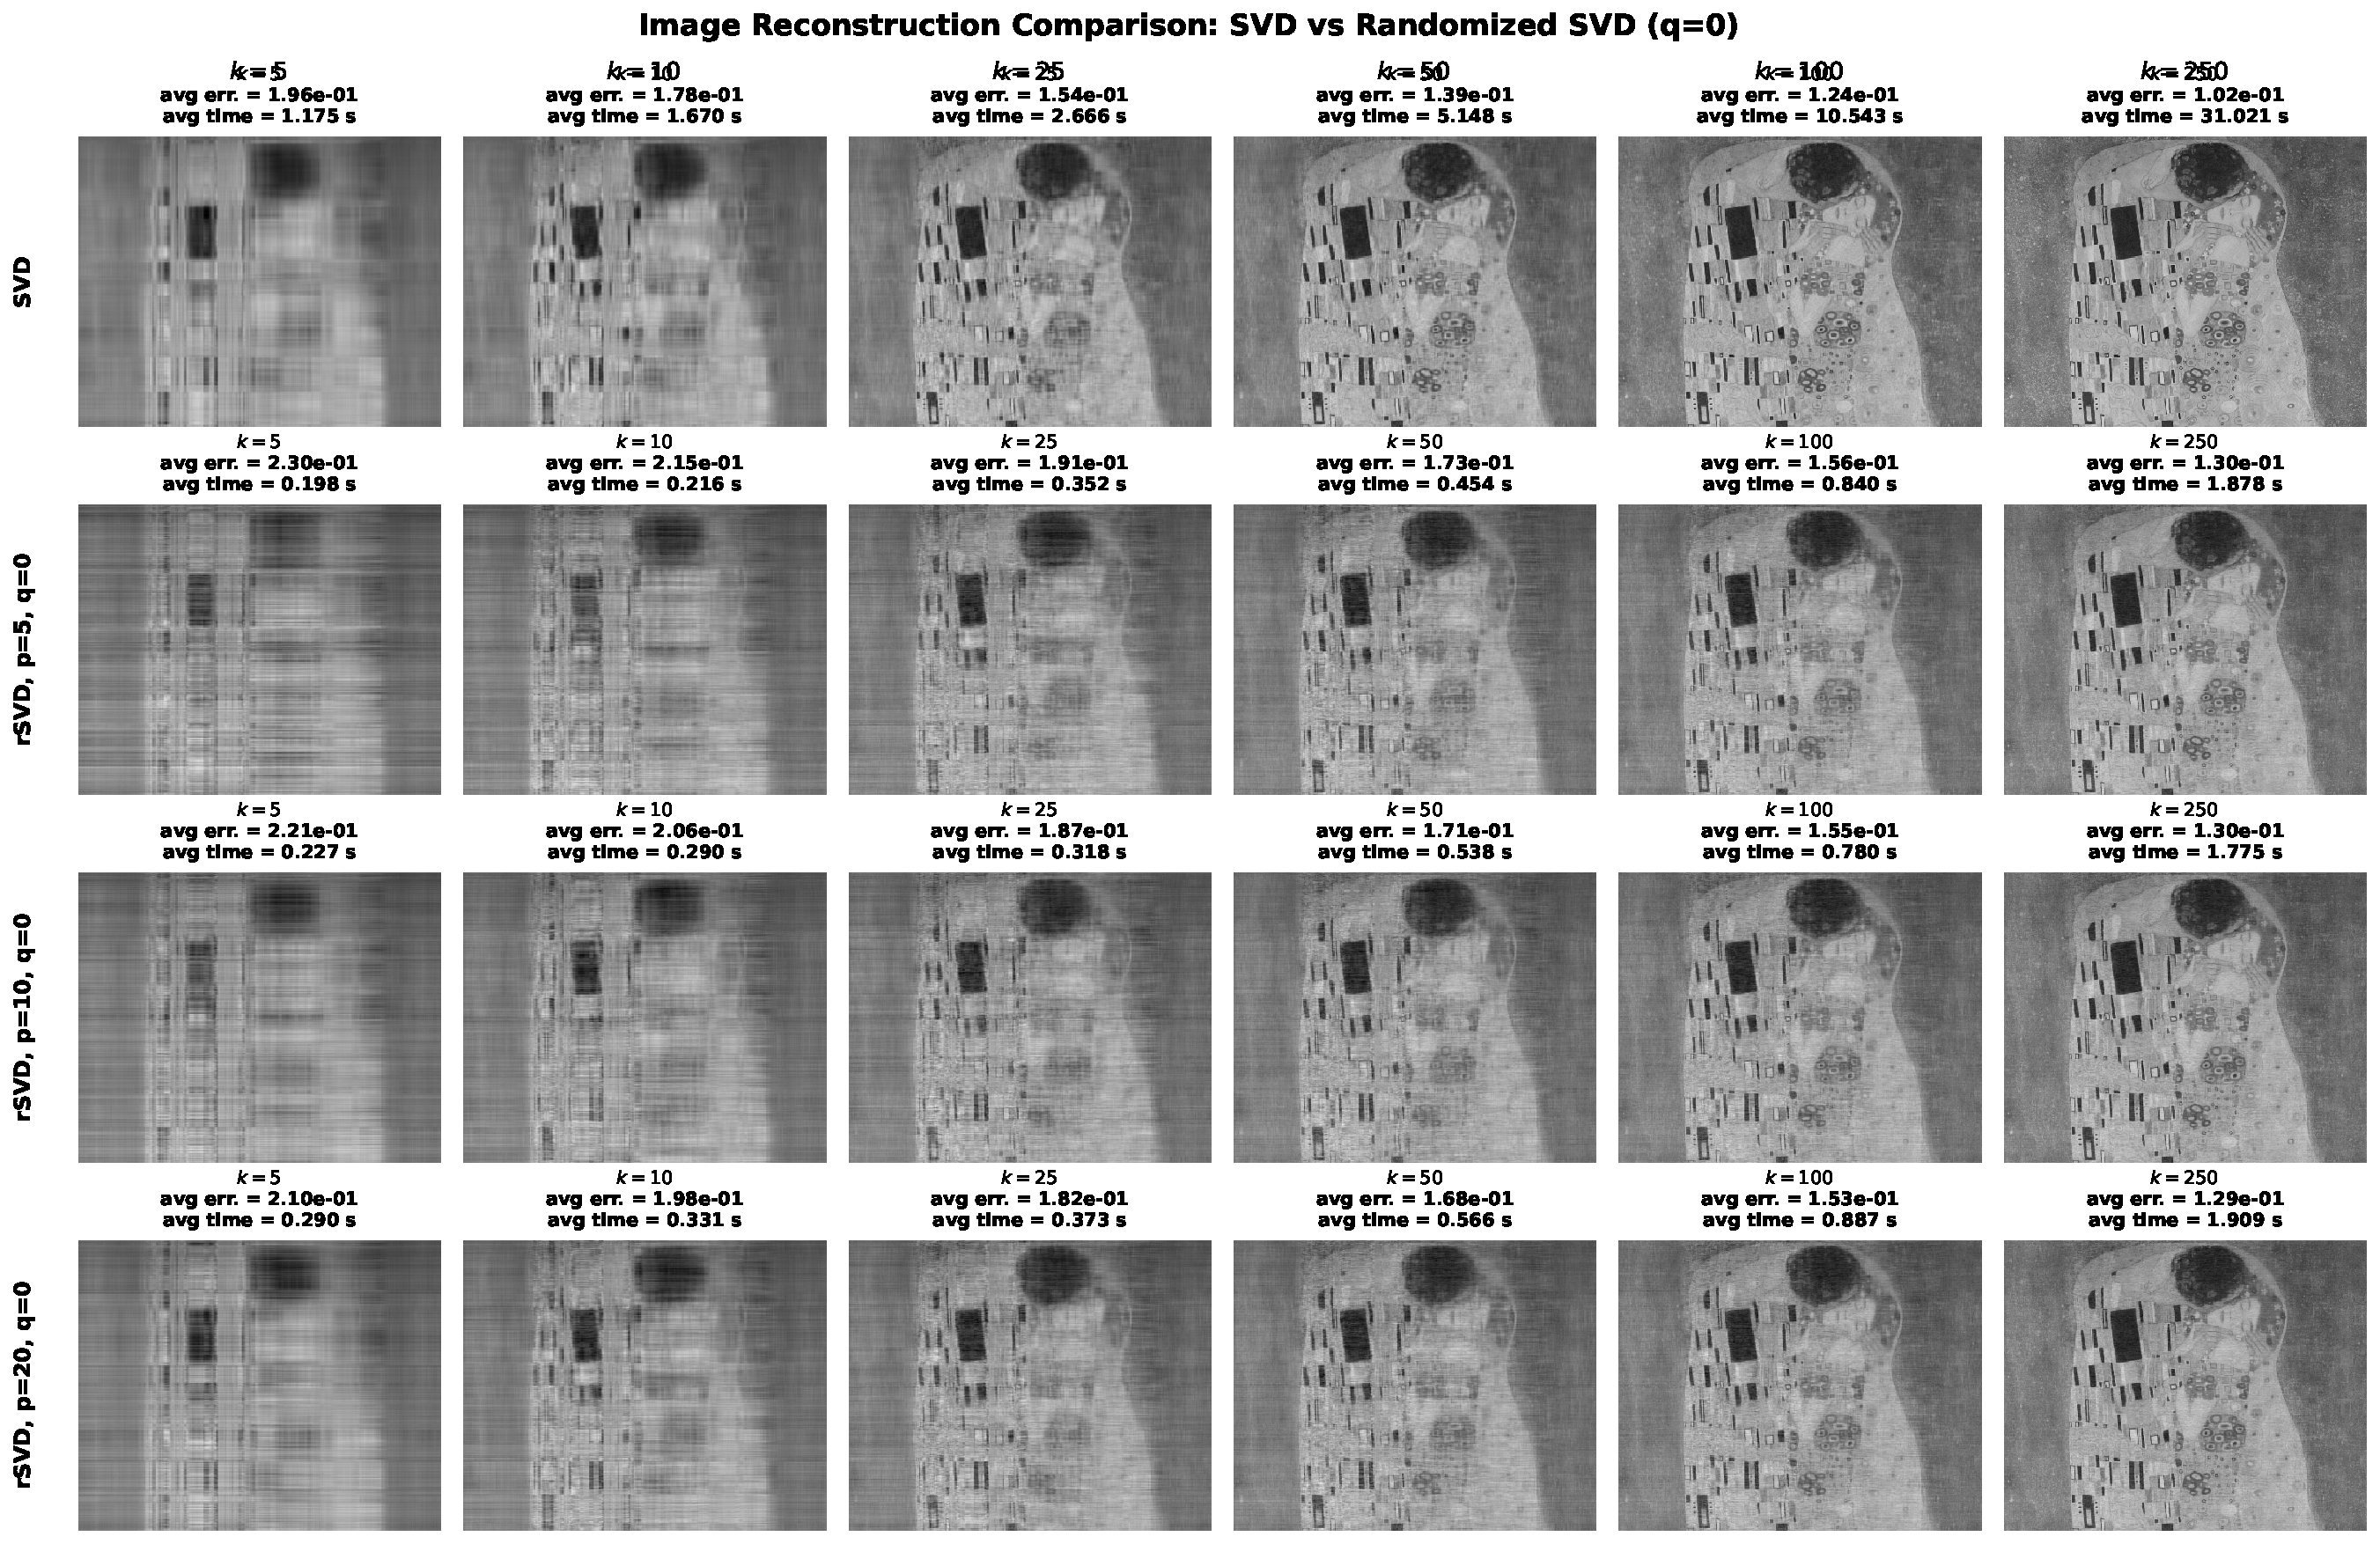
\includegraphics[width=1\textwidth,height=.85\textheight,keepaspectratio]{figures/svd_rsvd_image_reconstruction_q0-2.pdf}
\end{frame}

% 9
\begin{frame}{rSVD per compressione immagini: risultati con q = 1}
\centering
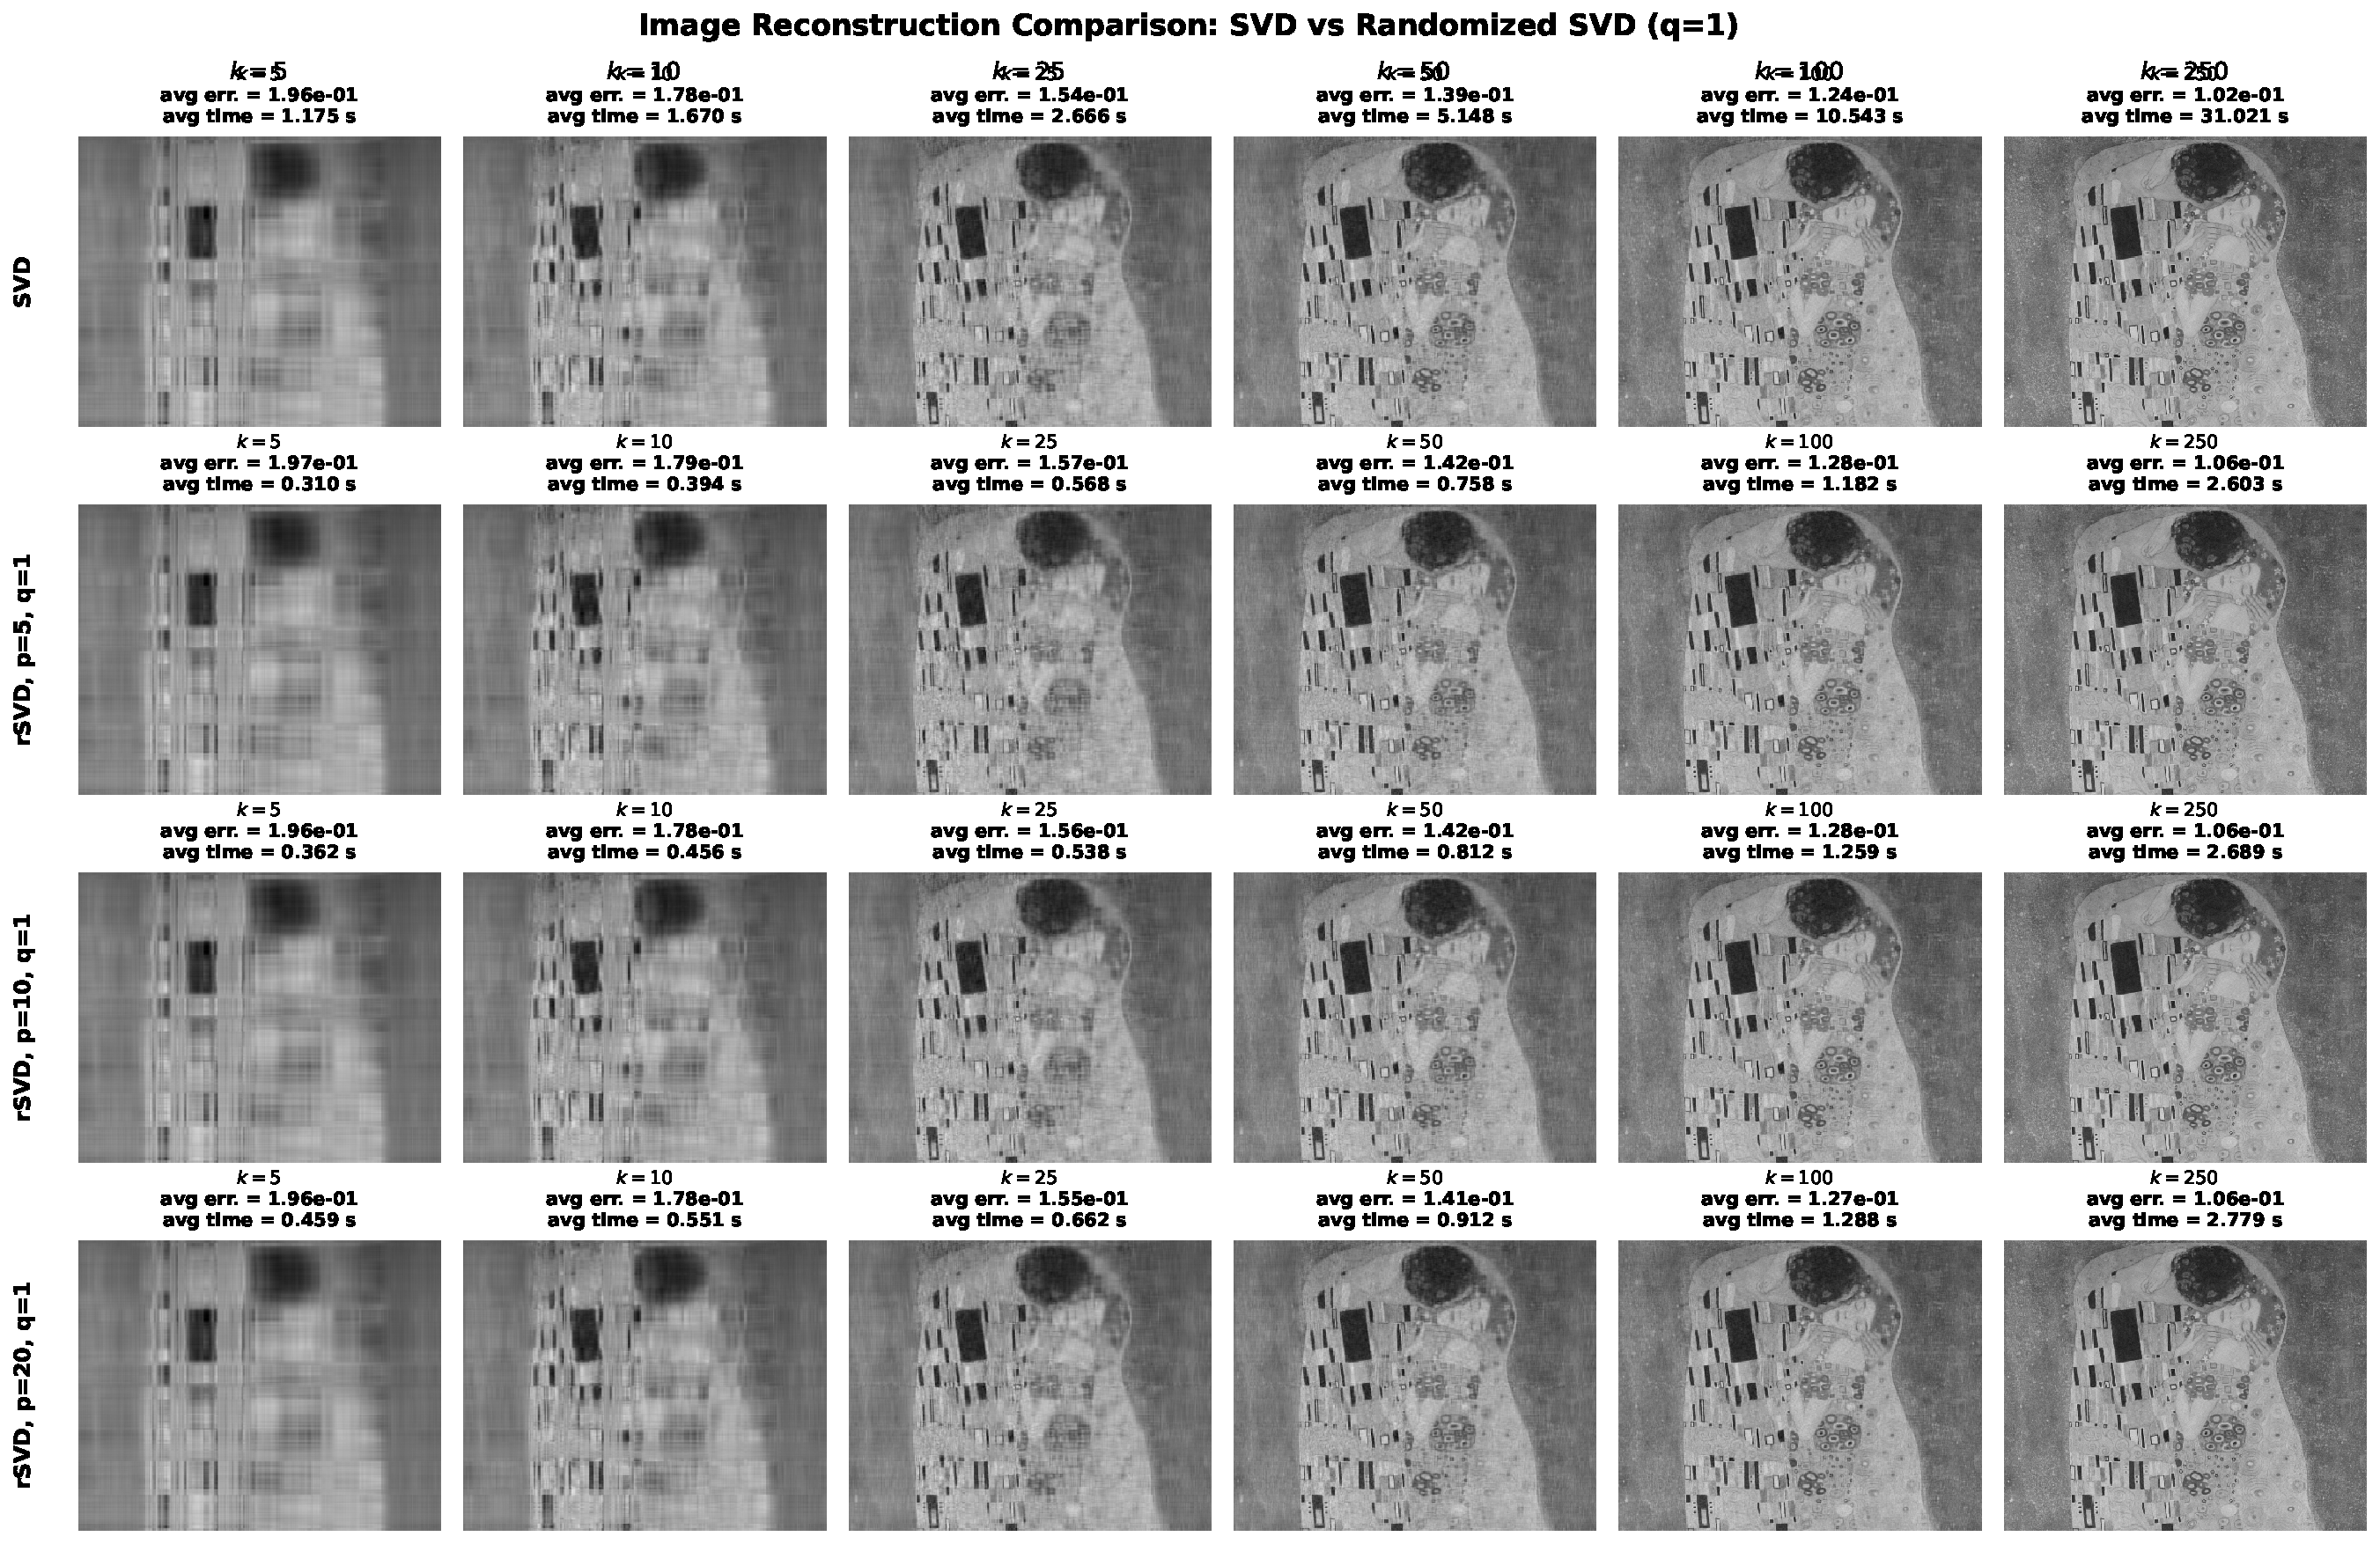
\includegraphics[width=1\textwidth,height=.85\textheight,keepaspectratio]{figures/svd_rsvd_image_reconstruction_q1.pdf}
\end{frame}

\begin{frame}{rSVD per compressione immagini: risultati}
\begin{columns}[T]
\column{0.50\textwidth}
\centering
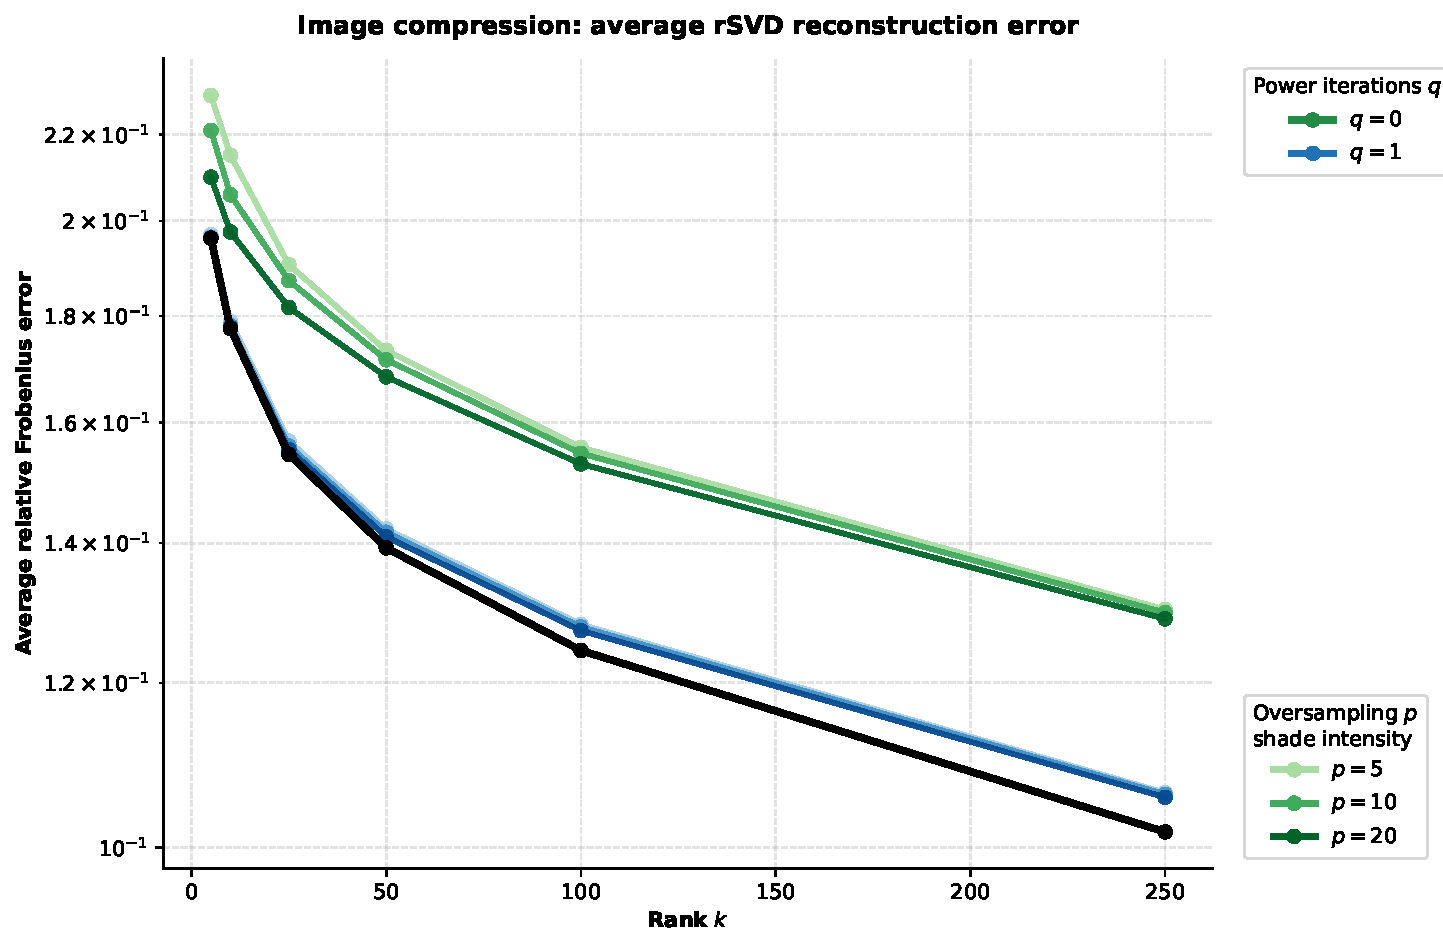
\includegraphics[width=\textwidth,height=0.55\textheight,keepaspectratio]{figures/rsvd_average_error_vs_rank.pdf}
\column{0.50\textwidth}
\centering
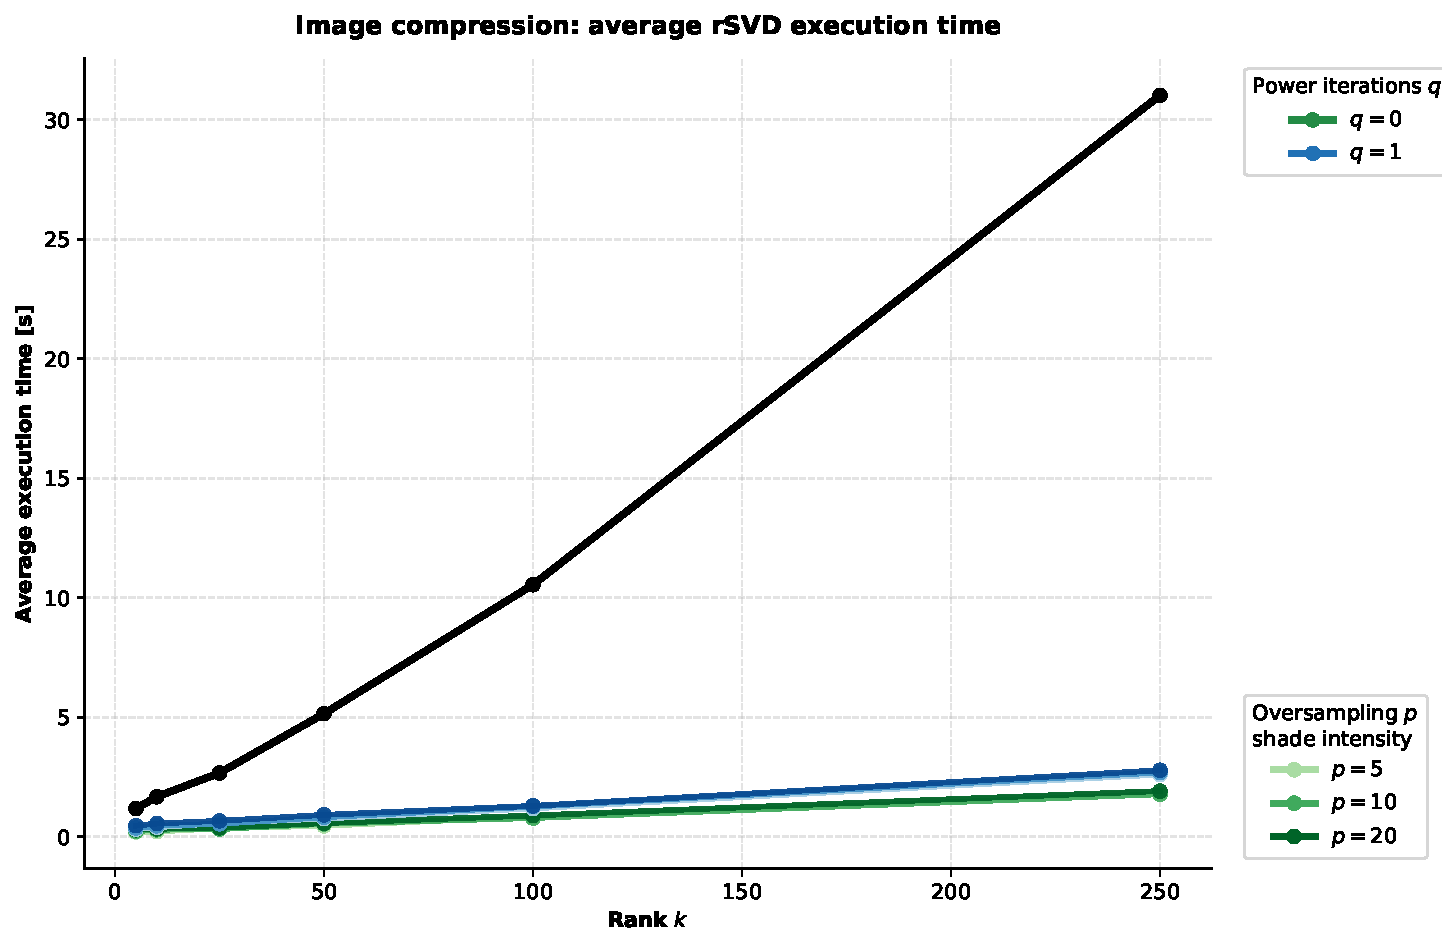
\includegraphics[width=\textwidth,height=0.55\textheight,keepaspectratio]{figures/rsvd_average_time_vs_rank.pdf}
\end{columns}
\vspace{0.1cm}
\begin{itemize}
  \item q=1 migliora l’accuratezza rispetto a q=0, con un costo leggermente maggiore.
  \item rSVD è molto più veloce della SVD classica, soprattutto per ranghi alti, mantenendo errori comparabili.
\end{itemize}
\end{frame}

% 10
\begin{frame}{rSVD per POD e POD-DEIM: introduzione}
Le PDE non lineari discretizzate generano sistemi ad altissima dimensione:
\[
\dot y(t)=Ay(t)+F(t,y(t)), \qquad y(t)\in\mathbb{R}^{d}, \quad d\gg 1.
\]
\begin{itemize}
  \item \textbf{POD}: riduce la dimensione dello stato costruendo una base dai dati.
  \item \textbf{rSVD}: accelera la costruzione offline delle basi POD.
  \item \textbf{DEIM}: riduce il costo online della valutazione del termine non lineare.
\end{itemize}
\begin{block}{Pipeline del notebook}
Full Order Model $\rightarrow$ snapshots di stato e nonlinear snapshots $\rightarrow$ basi POD/rPOD $\rightarrow$ punti DEIM $\rightarrow$ confronto train/test.
\end{block}
\end{frame}

% 11
\begin{frame}{Definizione POD}
Date le snapshots di soluzione
\[
y(t_0),\,y(t_1),\,\ldots,\,y(t_{N-1})\in\mathbb{R}^{d},
\]
si costruisce la snapshot matrix
\[
Y=\begin{bmatrix}y(t_0)&y(t_1)&\cdots&y(t_{N-1})\end{bmatrix}
\in\mathbb{R}^{d\times N}.
\]
Applicando la SVD:
\[
Y=U\Sigma V^T.
\]
La matrice delle basi POD di dimensione $r$ e' formata dai primi $r$ vettori singolari sinistri:
\[
\Psi=\begin{bmatrix}\psi_1&\psi_2&\cdots&\psi_r\end{bmatrix}\in\mathbb{R}^{d\times r}.
\]
La soluzione viene approssimata come
\[
y(t)\approx \Psi y^r(t),
\]
dove $y^r(t)\in\mathbb{R}^{r}$ e' lo stato ridotto.
\end{frame}

% 12
\begin{frame}{Definizione POD-DEIM}
Per il termine non lineare si raccolgono le nonlinear snapshots:
\[
F(t_0,y(t_0)),\,F(t_1,y(t_1)),\,\ldots,\,F(t_{N-1},y(t_{N-1})).
\]
Nel codice sono memorizzate nella matrice
\[
\widehat F=
\begin{bmatrix}
F(t_0,y(t_0))&F(t_1,y(t_1))&\cdots&F(t_{N-1},y(t_{N-1}))
\end{bmatrix}.
\]
Dalla SVD di $\widehat F$ si ottiene la matrice delle basi DEIM:
\[
\Phi=\begin{bmatrix}\phi_1&\phi_2&\cdots&\phi_m\end{bmatrix}\in\mathbb{R}^{d\times m}.
\]
DEIM approssima il termine non lineare come
\[
F(t,y(t))\approx \Phi c(t).
\]
\end{frame}

% 13
\begin{frame}{Scelta di $P$ e calcolo di $c(t)$}
La matrice $P\in\mathbb{R}^{d\times m}$ seleziona $m$ componenti del vettore non lineare:
\[
P=\begin{bmatrix}e_{\rho_1}&e_{\rho_2}&\cdots&e_{\rho_m}\end{bmatrix}.
\]
Nel notebook gli indici $\rho_i$ sono scelti con l'algoritmo greedy DEIM:
\begin{enumerate}
  \item $\rho_1=\arg\max_j|\phi_1(j)|$;
  \item per $i=2,\ldots,m$ si risolve
  \[
  (P_{i-1}^T\Phi_{i-1})c=P_{i-1}^T\phi_i,
  \]
  si calcola il residuo $r_i=\phi_i-\Phi_{i-1}c$;
  \item si sceglie $\rho_i=\arg\max_j|r_i(j)|$.
\end{enumerate}
Applicando $P^T$ a $F(t,y(t))\approx\Phi c(t)$:
\[
c(t)=(P^T\Phi)^{-1}P^TF(t,y(t)).
\]
\end{frame}

% 14
\begin{frame}{Fase offline, fase online ed errori}
\begin{block}{Offline}
Si risolve il full order model, si costruiscono $Y$ e $\widehat F$, si calcolano $\Psi$, $\Phi$ e gli indici DEIM. Nel notebook le basi sono costruite solo con il \textbf{training set}.
\end{block}
\begin{block}{Online}
Si usa il modello ridotto o l'approssimazione DEIM su dati non necessariamente gia' visti. La dimensione e' $r$ per POD e $m$ punti per DEIM.
\end{block}
\begin{itemize}
  \item \textbf{Errore train/offline POD}:
  \[
  E_{\mathrm{train}}^{\mathrm{POD}}=
  \frac{\|Y_{\mathrm{train}}-\Psi\Psi^TY_{\mathrm{train}}\|_F}{\|Y_{\mathrm{train}}\|_F}.
  \]
  \item \textbf{Errore test/online POD}: stessa formula su $Y_{\mathrm{test}}$, non usata per costruire $\Psi$.
  \item \textbf{Errore train/test DEIM}: media degli errori relativi
  \[
  E^{\mathrm{DEIM}}=
  \frac{\|F(t_j,y_j)-\Phi(P^T\Phi)^{-1}P^TF(t_j,y_j)\|_2}{\|F(t_j,y_j)\|_2}.
  \]
\end{itemize}
\end{frame}


% 15
\begin{frame}{Allen--Cahn: definizione del problema}
La prima PDE testata e' l'equazione di Allen--Cahn:
\[
y_t(x,t)-\alpha\Delta y(x,t)-\mu\left(y(x,t)-y^3(x,t)\right)=0,
\qquad \Omega=(0,1)^2.
\]
Condizioni al bordo omogenee di Dirichlet e condizione iniziale:
\[
y(x_1,x_2,0)=0.1\sin(\pi x_1)\sin(\pi x_2).
\]
Parametri sperimentali:
\[
\alpha=0.1,\quad \mu=11,\quad T=5,\quad n=256,\quad d=256^2=65536.
\]
\[
\Delta t=0.005,\qquad \text{snapshot stride}=5.
\]
La matrice degli snapshots ha dimensione $65536\times201$.
\centering
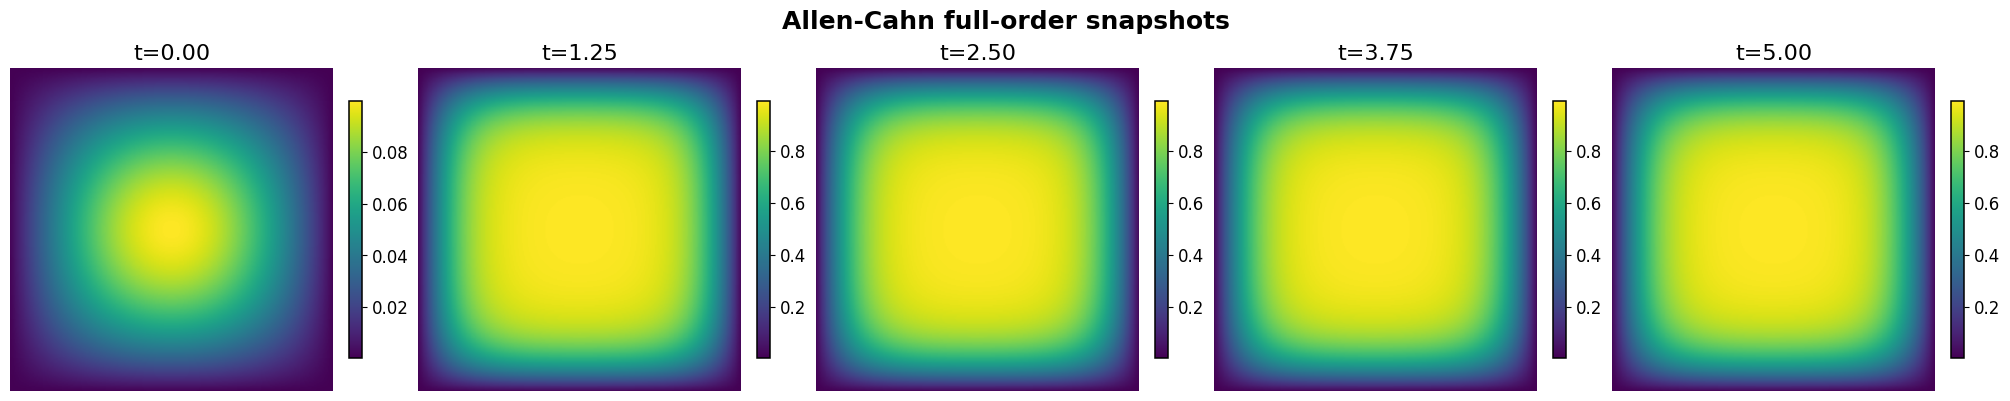
\includegraphics[width=0.72\textwidth,height=0.24\textheight,keepaspectratio]{figures/ac.png}
\end{frame}

% 16
\begin{frame}{Allen--Cahn: full order model e snapshots}
Sul reticolo dei punti interni si costruisce il Laplaciano sparso $L$ con differenze finite centrate.
L'equazione e' integrata con schema semi-implicito:
\[
(I-\Delta t\,\alpha L)y^{n+1}
=
y^n+\Delta t\,\mu\left(y^n-(y^n)^3\right).
\]
\begin{itemize}
  \item La matrice $I-\Delta t\,\alpha L$ e' fattorizzata una sola volta.
  \item Ogni 5 passi temporali si salva una colonna di $Y$.
  \item Gli snapshots sono divisi nel notebook in $70\%$ train e $30\%$ test.
\end{itemize}
\begin{block}{Snapshot matrix}
\[
Y_{\mathrm{AC}}=\begin{bmatrix}y(t_0)&\cdots&y(t_{200})\end{bmatrix}
\in\mathbb{R}^{65536\times201}.
\]
\end{block}
\end{frame}

% 17
\begin{frame}{Risultati Allen--Cahn: POD}
\begin{columns}[T]

\column{0.33\textwidth}
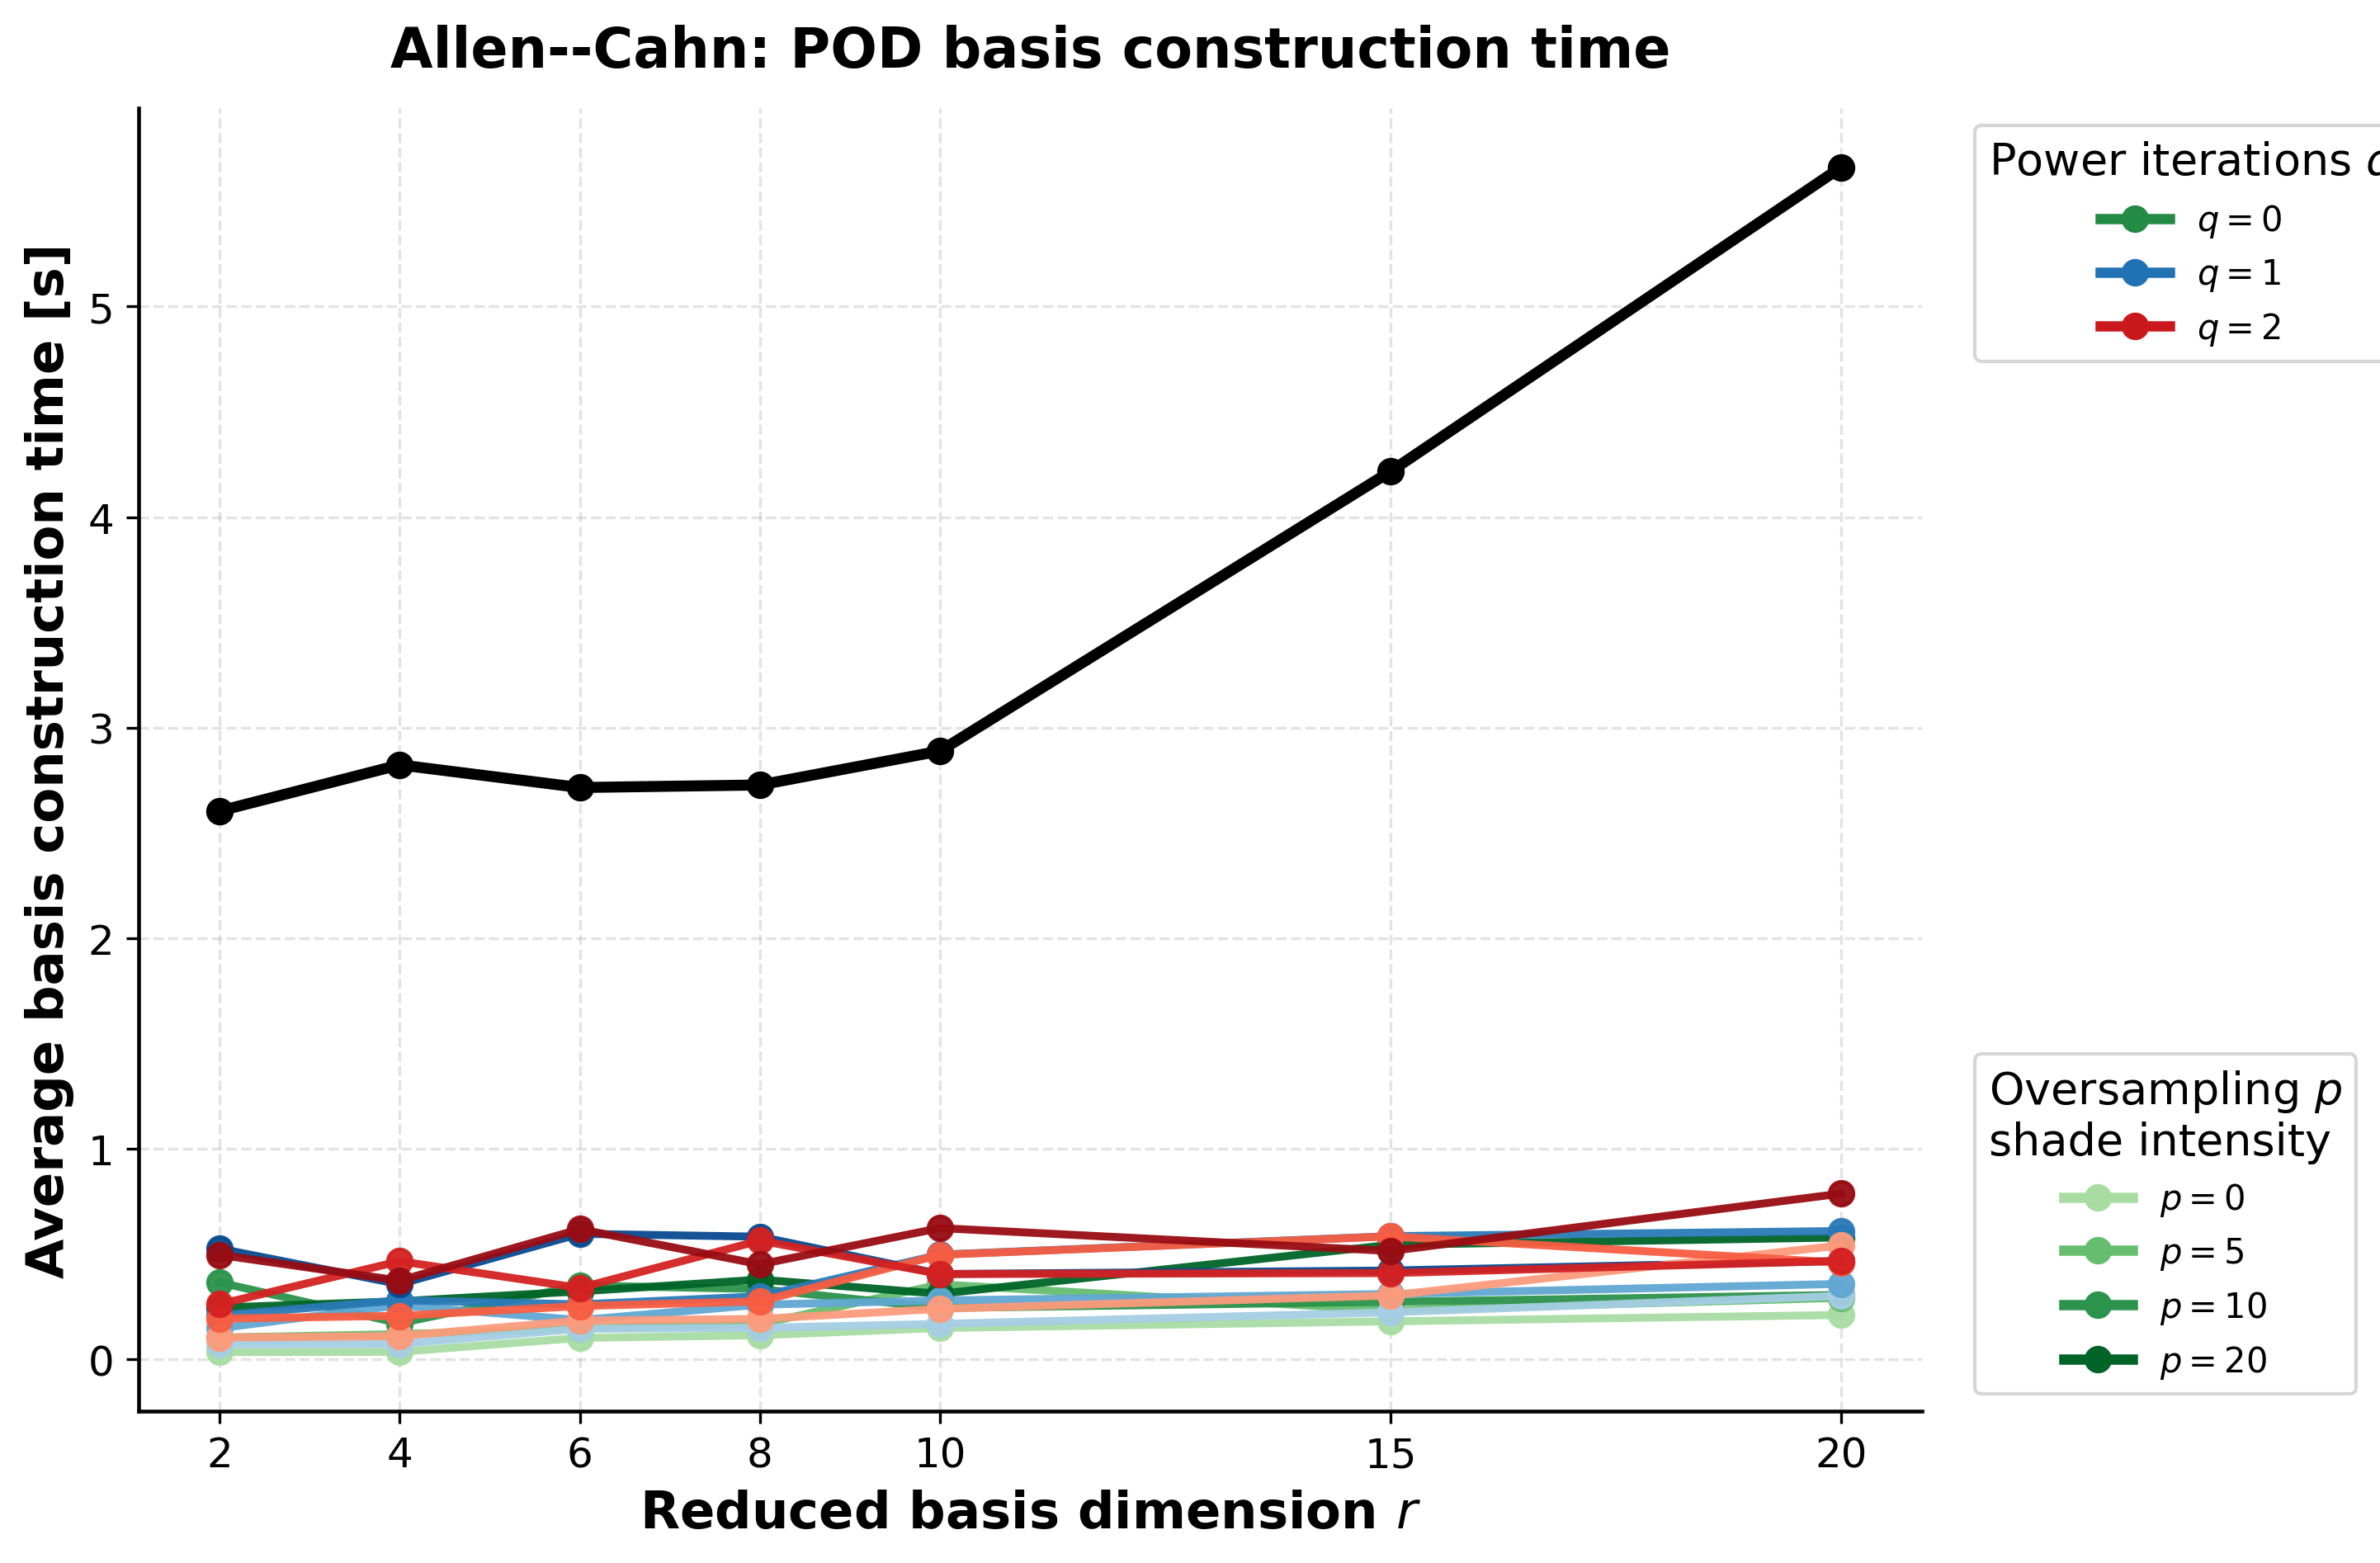
\includegraphics[width=\textwidth,height=0.42\textheight,keepaspectratio]{figures/allen_cahn_pod_basis_time.png}

\column{0.33\textwidth}
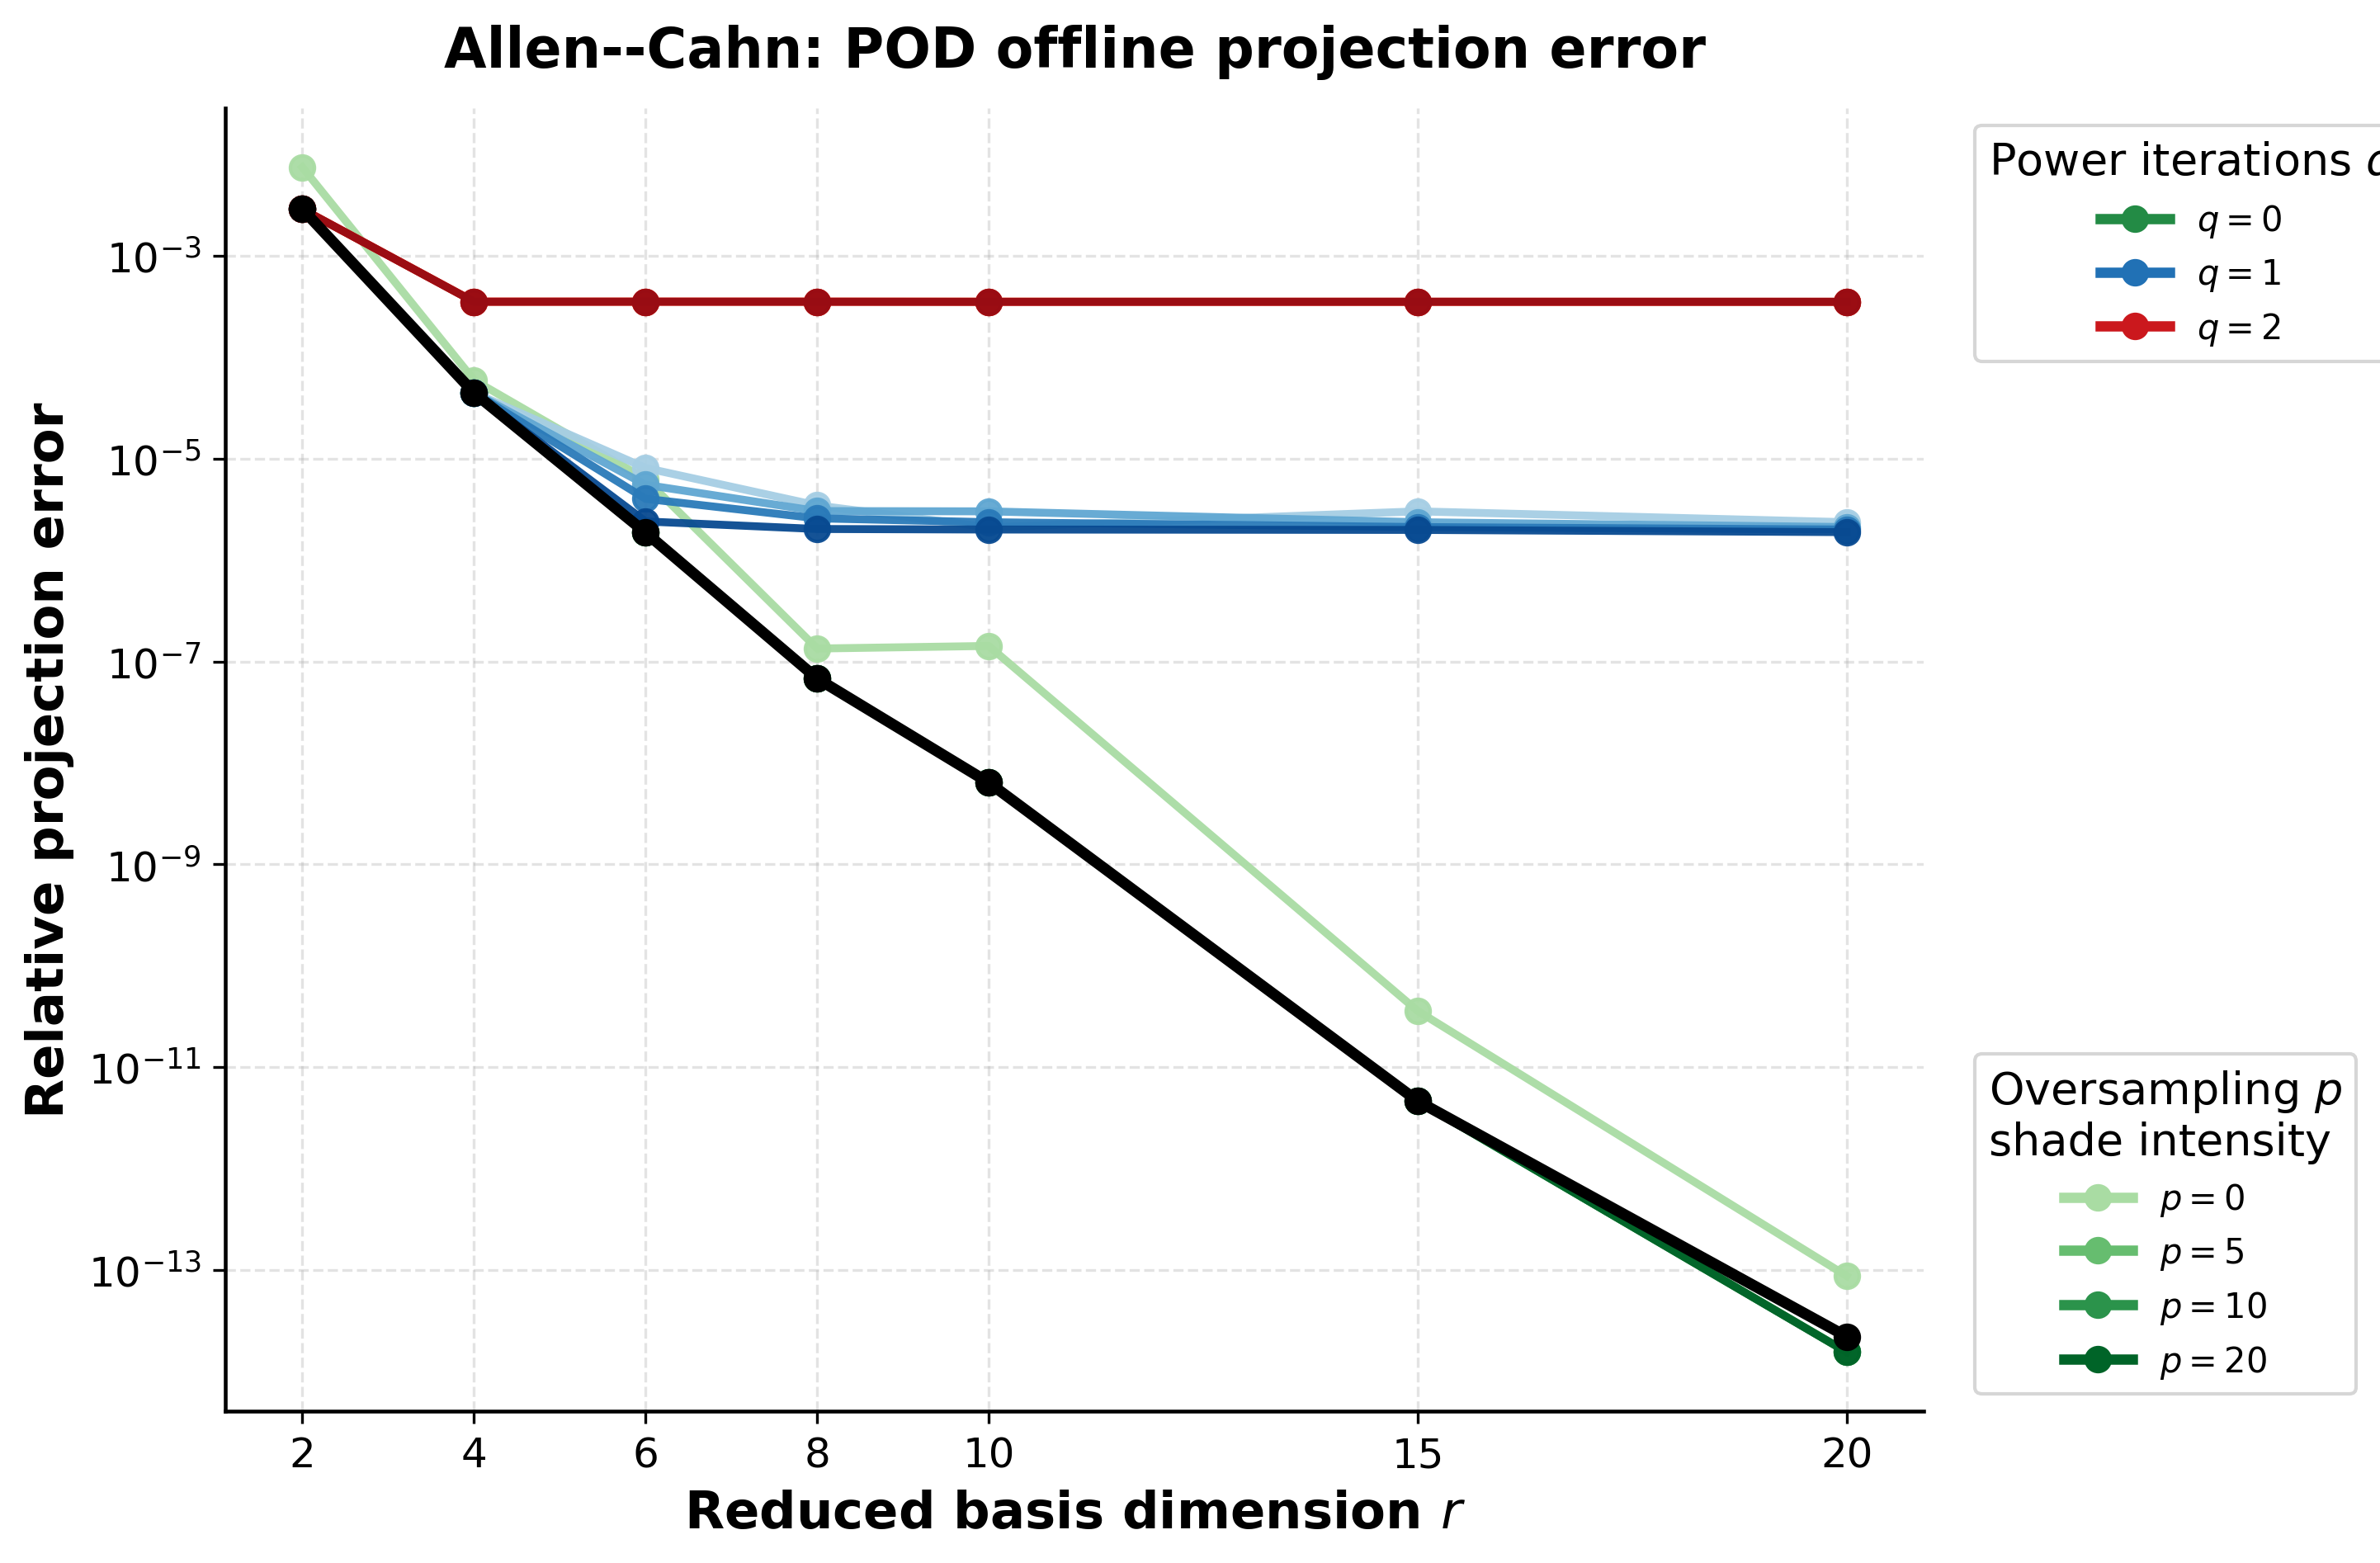
\includegraphics[width=\textwidth,height=0.42\textheight,keepaspectratio]{figures/allen_cahn_pod_offline_error.png}

\column{0.33\textwidth}
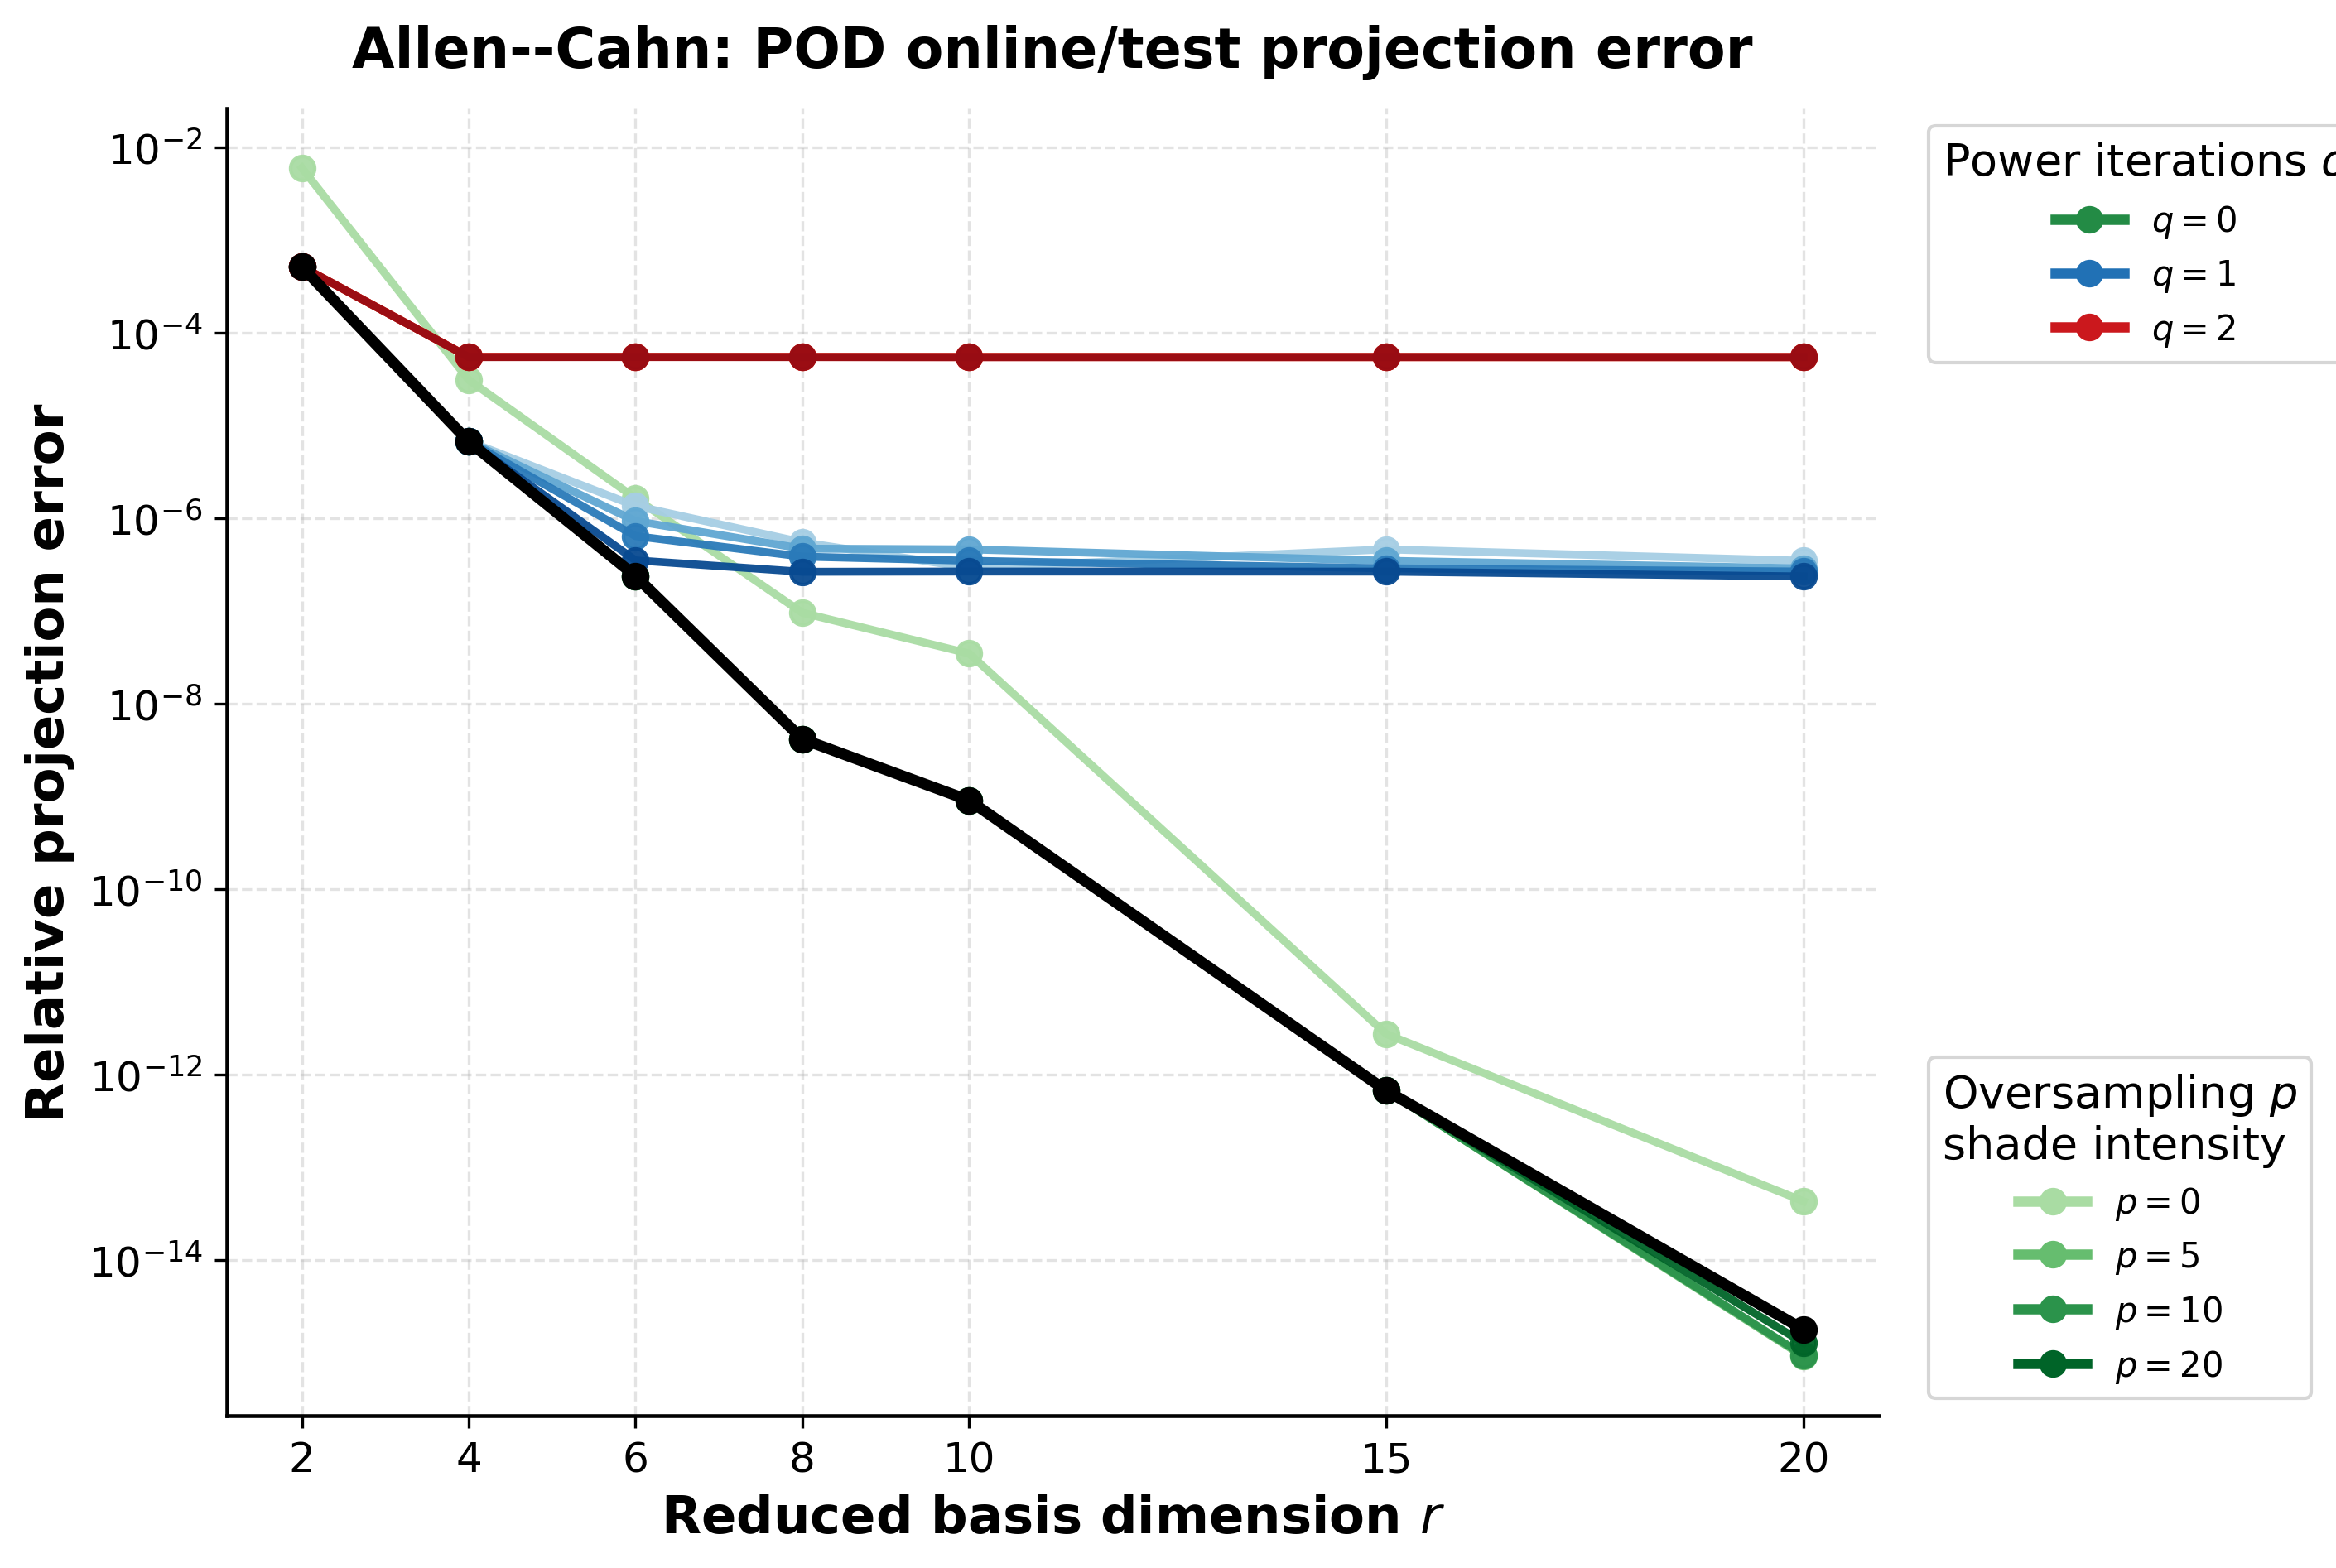
\includegraphics[width=\textwidth,height=0.42\textheight,keepaspectratio]{figures/allen_cahn_pod_online_error.png}

\end{columns}

\vspace{0.25cm}

\begin{block}{Lettura dei grafici}
\begin{itemize}
  \item La base e' costruita su $Y_{\mathrm{AC,train}}$.
  \item L'errore offline misura la ricostruzione delle snapshots di train.
  \item L'errore online/test misura la generalizzazione sulle snapshots temporali non usate nella base.
\end{itemize}
\end{block}

\end{frame}

% 18
\begin{frame}{Allen--Cahn: nonlinear snapshots per DEIM}
Per costruire la base DEIM non si usa direttamente $Y$, ma il termine non lineare:
\[
F(t,y(t))=\mu\left(y(t)-y(t)^3\right).
\]
Per ogni snapshot di stato salvato si calcola:
\[
F(t_j,y(t_j))=\mu\left(y(t_j)-y(t_j)^3\right),
\qquad j=0,\ldots,200.
\]
La matrice usata per la base DEIM e':
\[
\widehat F_{\mathrm{AC}}=
\begin{bmatrix}
F(t_0,y(t_0))&F(t_1,y(t_1))&\cdots&F(t_{200},y(t_{200}))
\end{bmatrix}.
\]
\begin{itemize}
  \item $\Phi$ e gli indici DEIM sono costruiti solo da $\widehat F_{\mathrm{AC,train}}$.
  \item L'errore online/test valuta l'approssimazione DEIM sugli stati $Y_{\mathrm{AC,test}}$.
\end{itemize}
\end{frame}

% 19
\begin{frame}{Risultati Allen--Cahn: POD-DEIM}
\begin{columns}[T]

\column{0.33\textwidth}
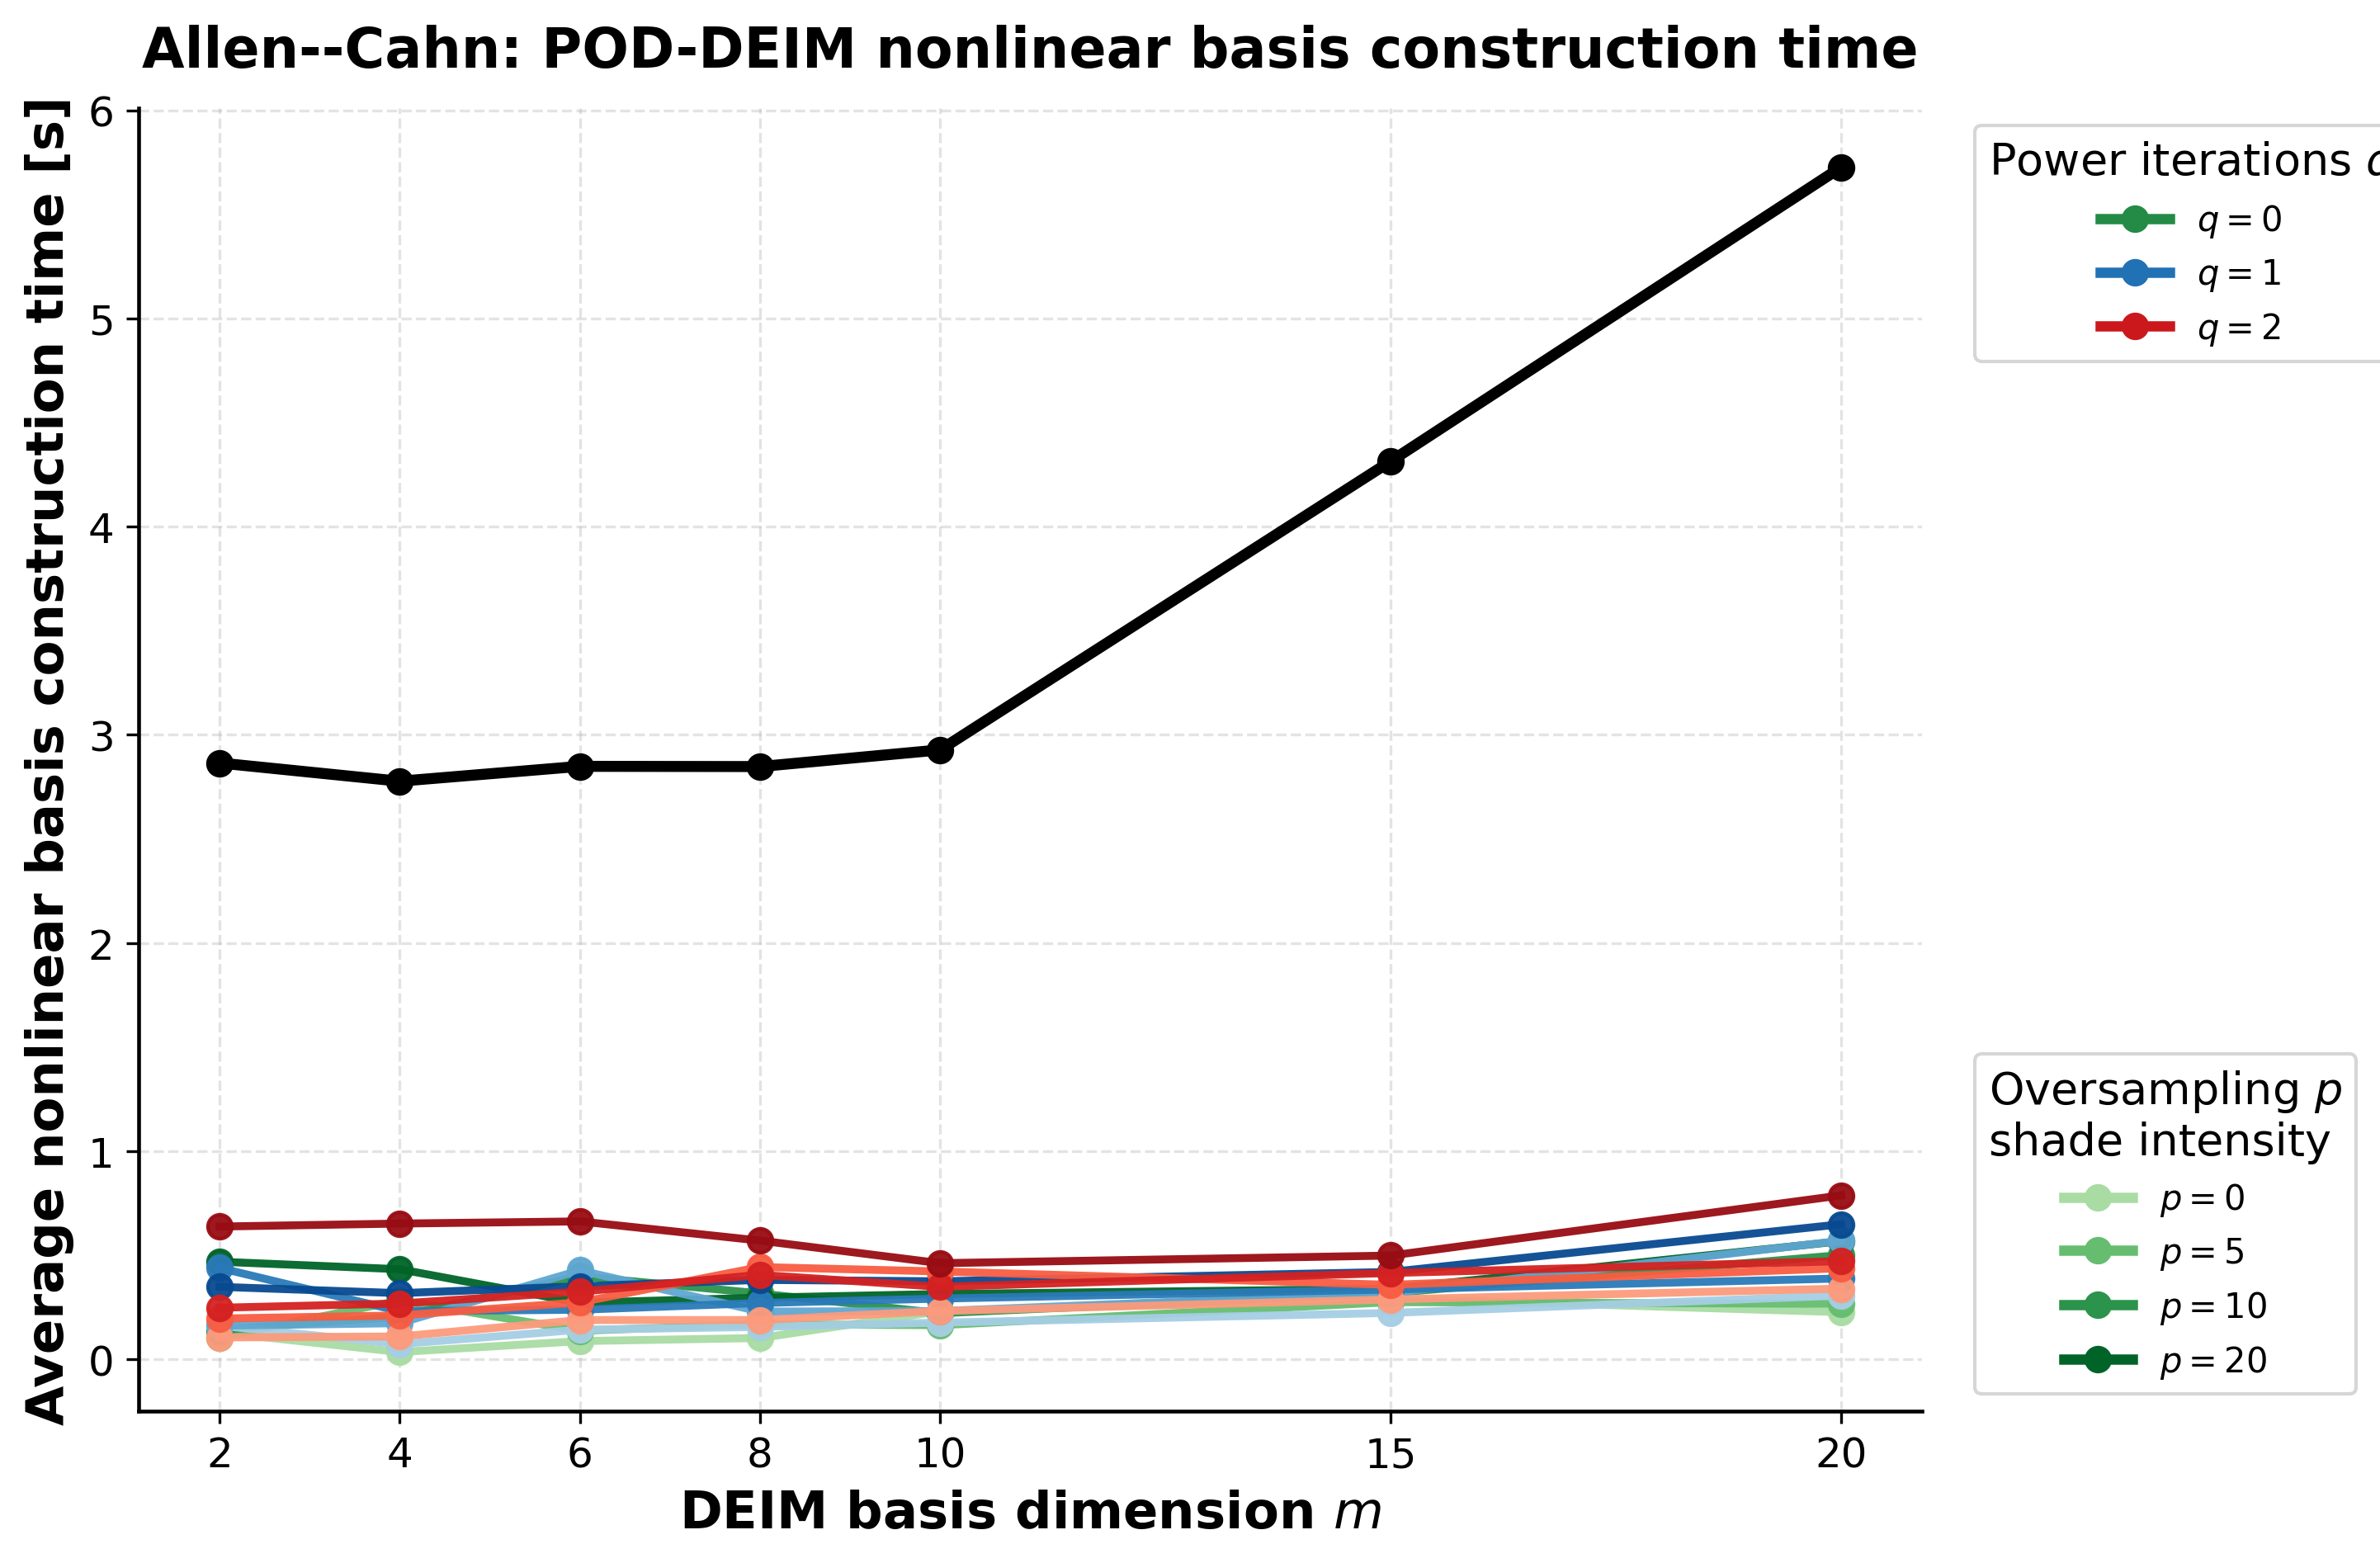
\includegraphics[width=\textwidth,height=0.42\textheight,keepaspectratio]{figures/allen_cahn_deim_basis_time.png}

\column{0.33\textwidth}
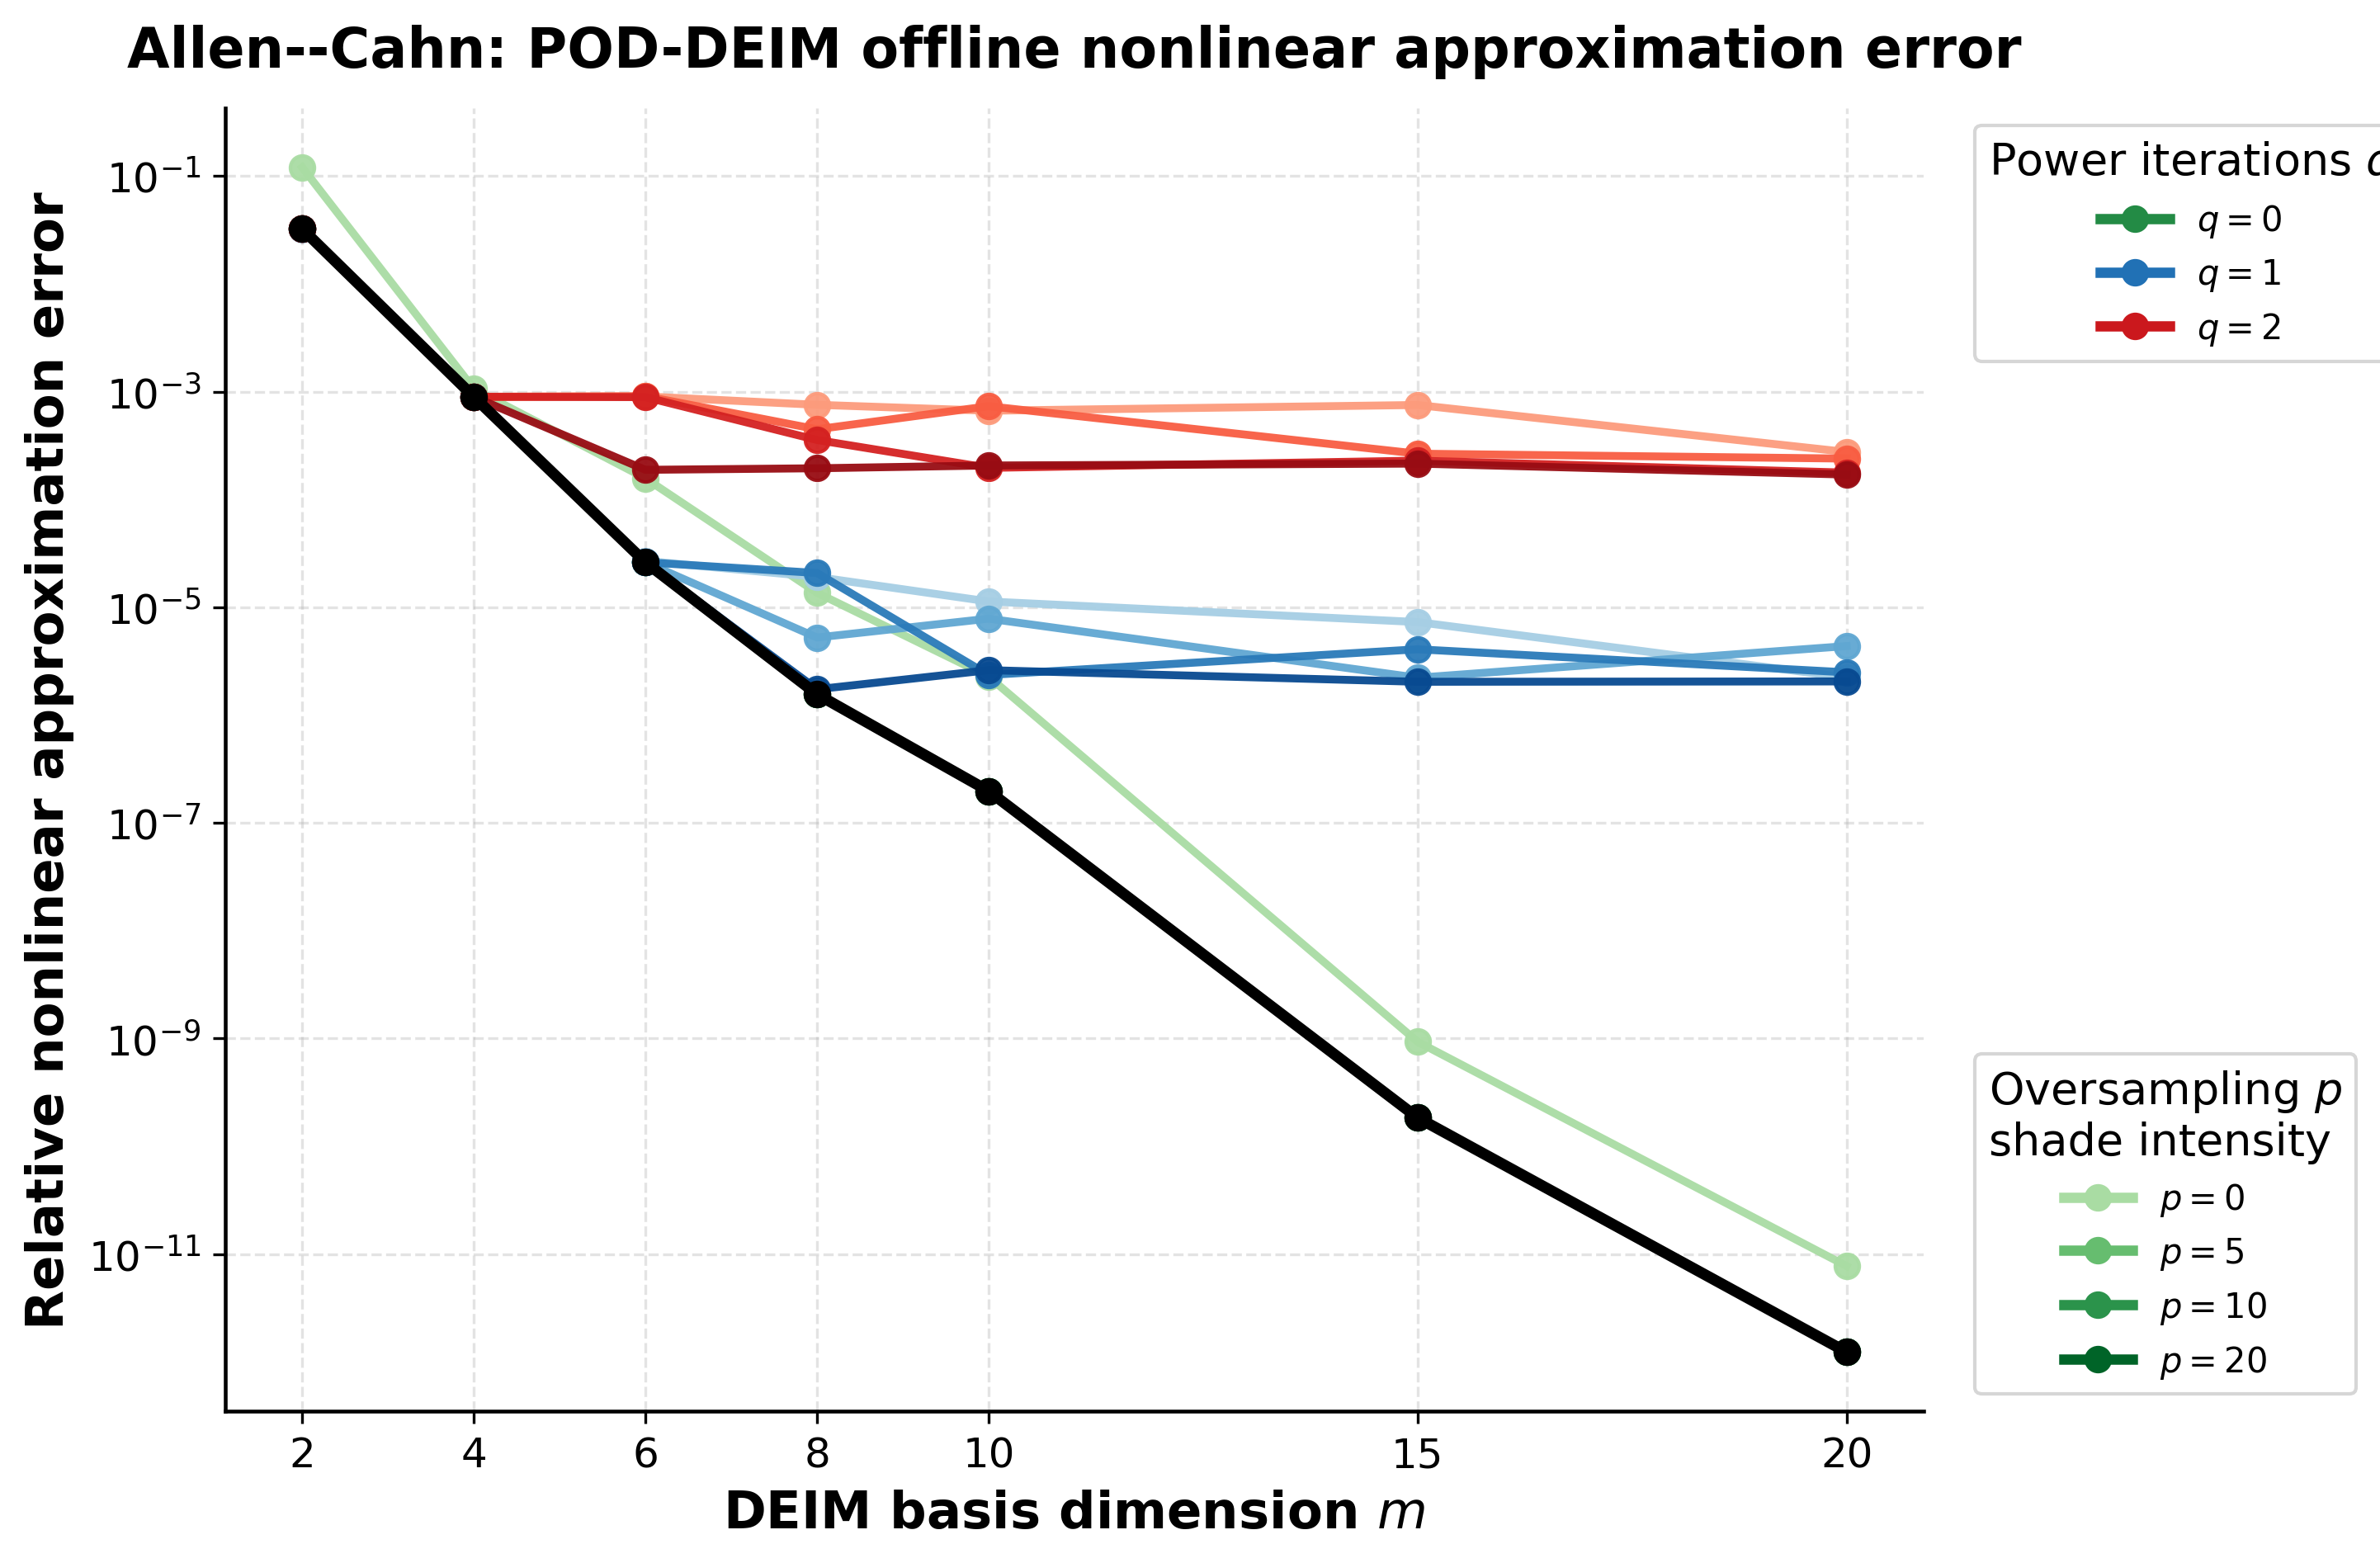
\includegraphics[width=\textwidth,height=0.42\textheight,keepaspectratio]{figures/allen_cahn_deim_offline_error.png}

\column{0.33\textwidth}
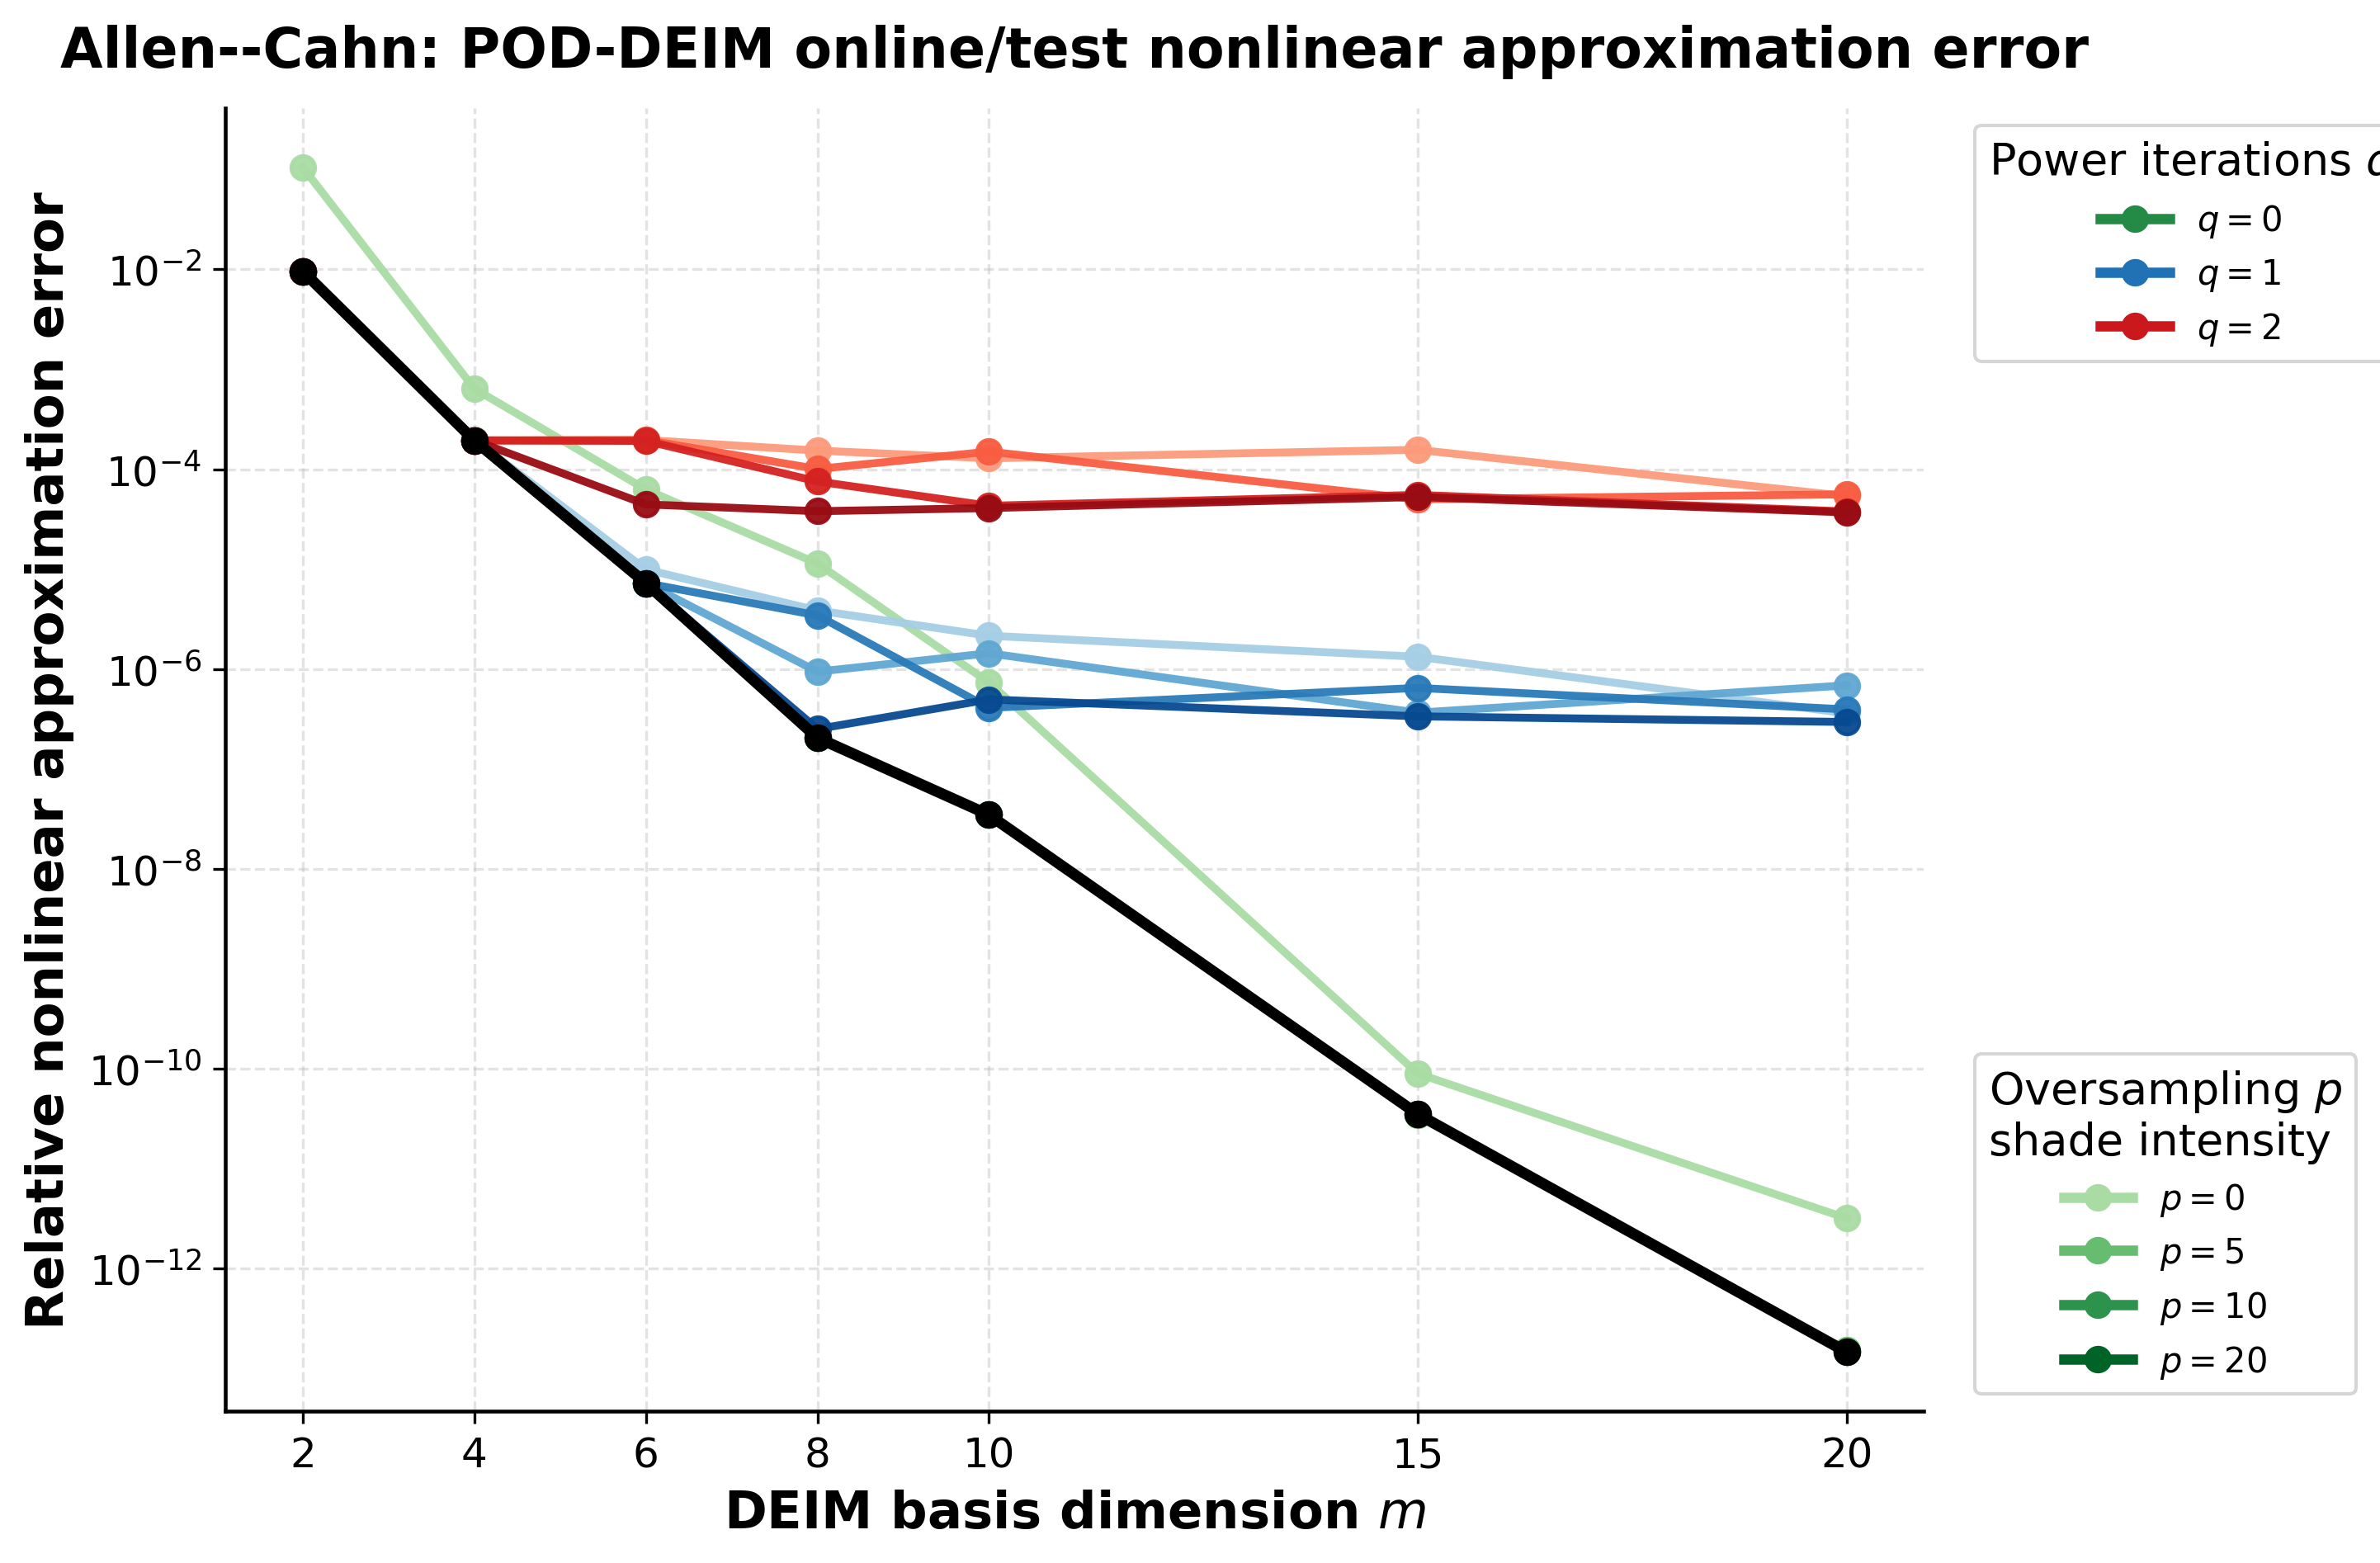
\includegraphics[width=\textwidth,height=0.42\textheight,keepaspectratio]{figures/allen_cahn_deim_online_error.png}

\end{columns}

\vspace{0.25cm}

\begin{block}{Lettura dei grafici}
\begin{itemize}
  \item La base non lineare e' calcolata da $\widehat F_{\mathrm{AC,train}}$.
  \item Il costo di costruzione riguarda $\Phi$; il costo online usa solo i punti selezionati da $P$.
  \item Gli errori mostrano la qualita' dell'approssimazione del termine non lineare.
\end{itemize}
\end{block}

\end{frame}

% 20
\begin{frame}{PDE ellittica stazionaria: definizione}
Il secondo benchmark e' una PDE ellittica stazionaria non lineare:
\[
-\nabla^2u(x,y)+s(u(x,y);\mu)=100\sin(2\pi x)\sin(2\pi y),
\]
con
\[
s(u;\mu)=\frac{\mu_1}{\mu_2}\left(e^{\mu_2u}-1\right),
\qquad
\mu=(\mu_1,\mu_2)\in[0.01,10]^2.
\]
Condizioni al bordo omogenee di Dirichlet. Parametri e dimensioni:
\begin{itemize}
  \item dominio $\Omega=(0,1)^2$, griglia $n=256$, quindi $d=65536$;
  \item griglia parametrica: $16\times16=256$ coppie $(\mu_1,\mu_2)$;
  \item snapshot matrix: $Y_{\mathrm{ell}}\in\mathbb{R}^{65536\times256}$.
\end{itemize}

\centering
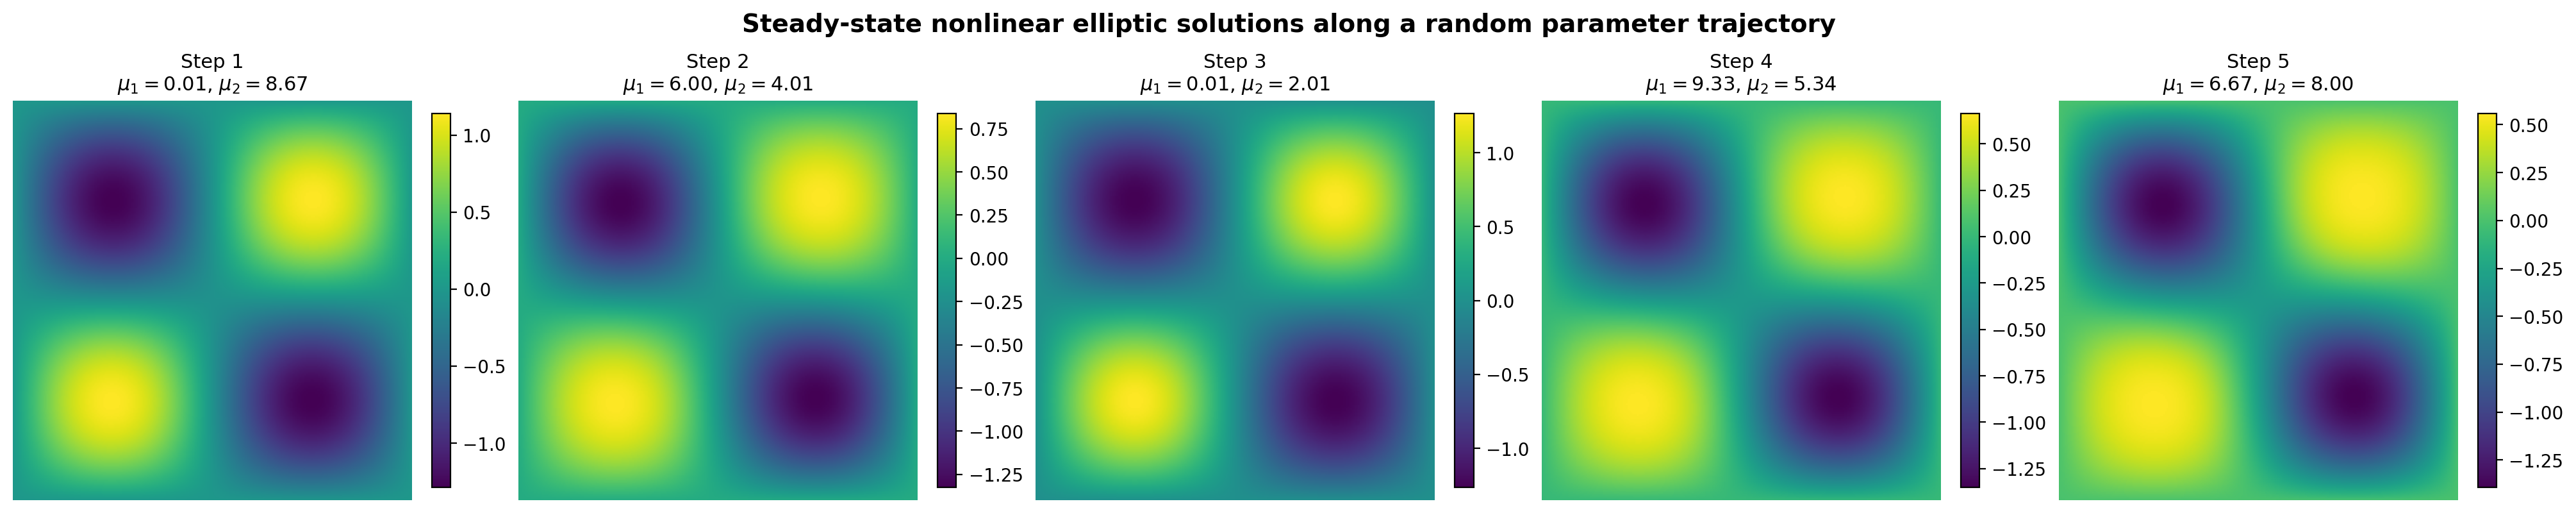
\includegraphics[width=0.72\textwidth,height=0.23\textheight,keepaspectratio]{figures/ell.png}

\end{frame}

% 21
\begin{frame}{PDE ellittica: full order model e snapshots}
Dopo la discretizzazione a differenze finite si risolve, per ogni coppia $\mu=(\mu_1,\mu_2)$, il sistema non lineare:
\[
R(u;\mu)=-Lu+s(u;\mu)-b=0,
\]
dove $b$ e' il termine sorgente discretizzato.
\begin{block}{Metodo di Newton usato nel codice}
Partendo da un guess iniziale, a ogni iterazione si risolve
\[
\left[-L+\operatorname{diag}\left(\mu_1 e^{\mu_2u}\right)\right]\delta u
=-R(u;\mu),
\qquad u\leftarrow u+\delta u.
\]
La tolleranza sul residuo relativo e' $10^{-10}$ e il massimo e' 30 iterazioni.
\end{block}
\begin{itemize}
  \item Il codice usa la soluzione precedente come initial guess per il parametro successivo.
  \item Gli snapshots sono divisi in $70\%$ train e $30\%$ test.
\end{itemize}
\end{frame}

% 22
\begin{frame}{Risultati PDE ellittica: POD}
\begin{columns}[T]

\column{0.33\textwidth}
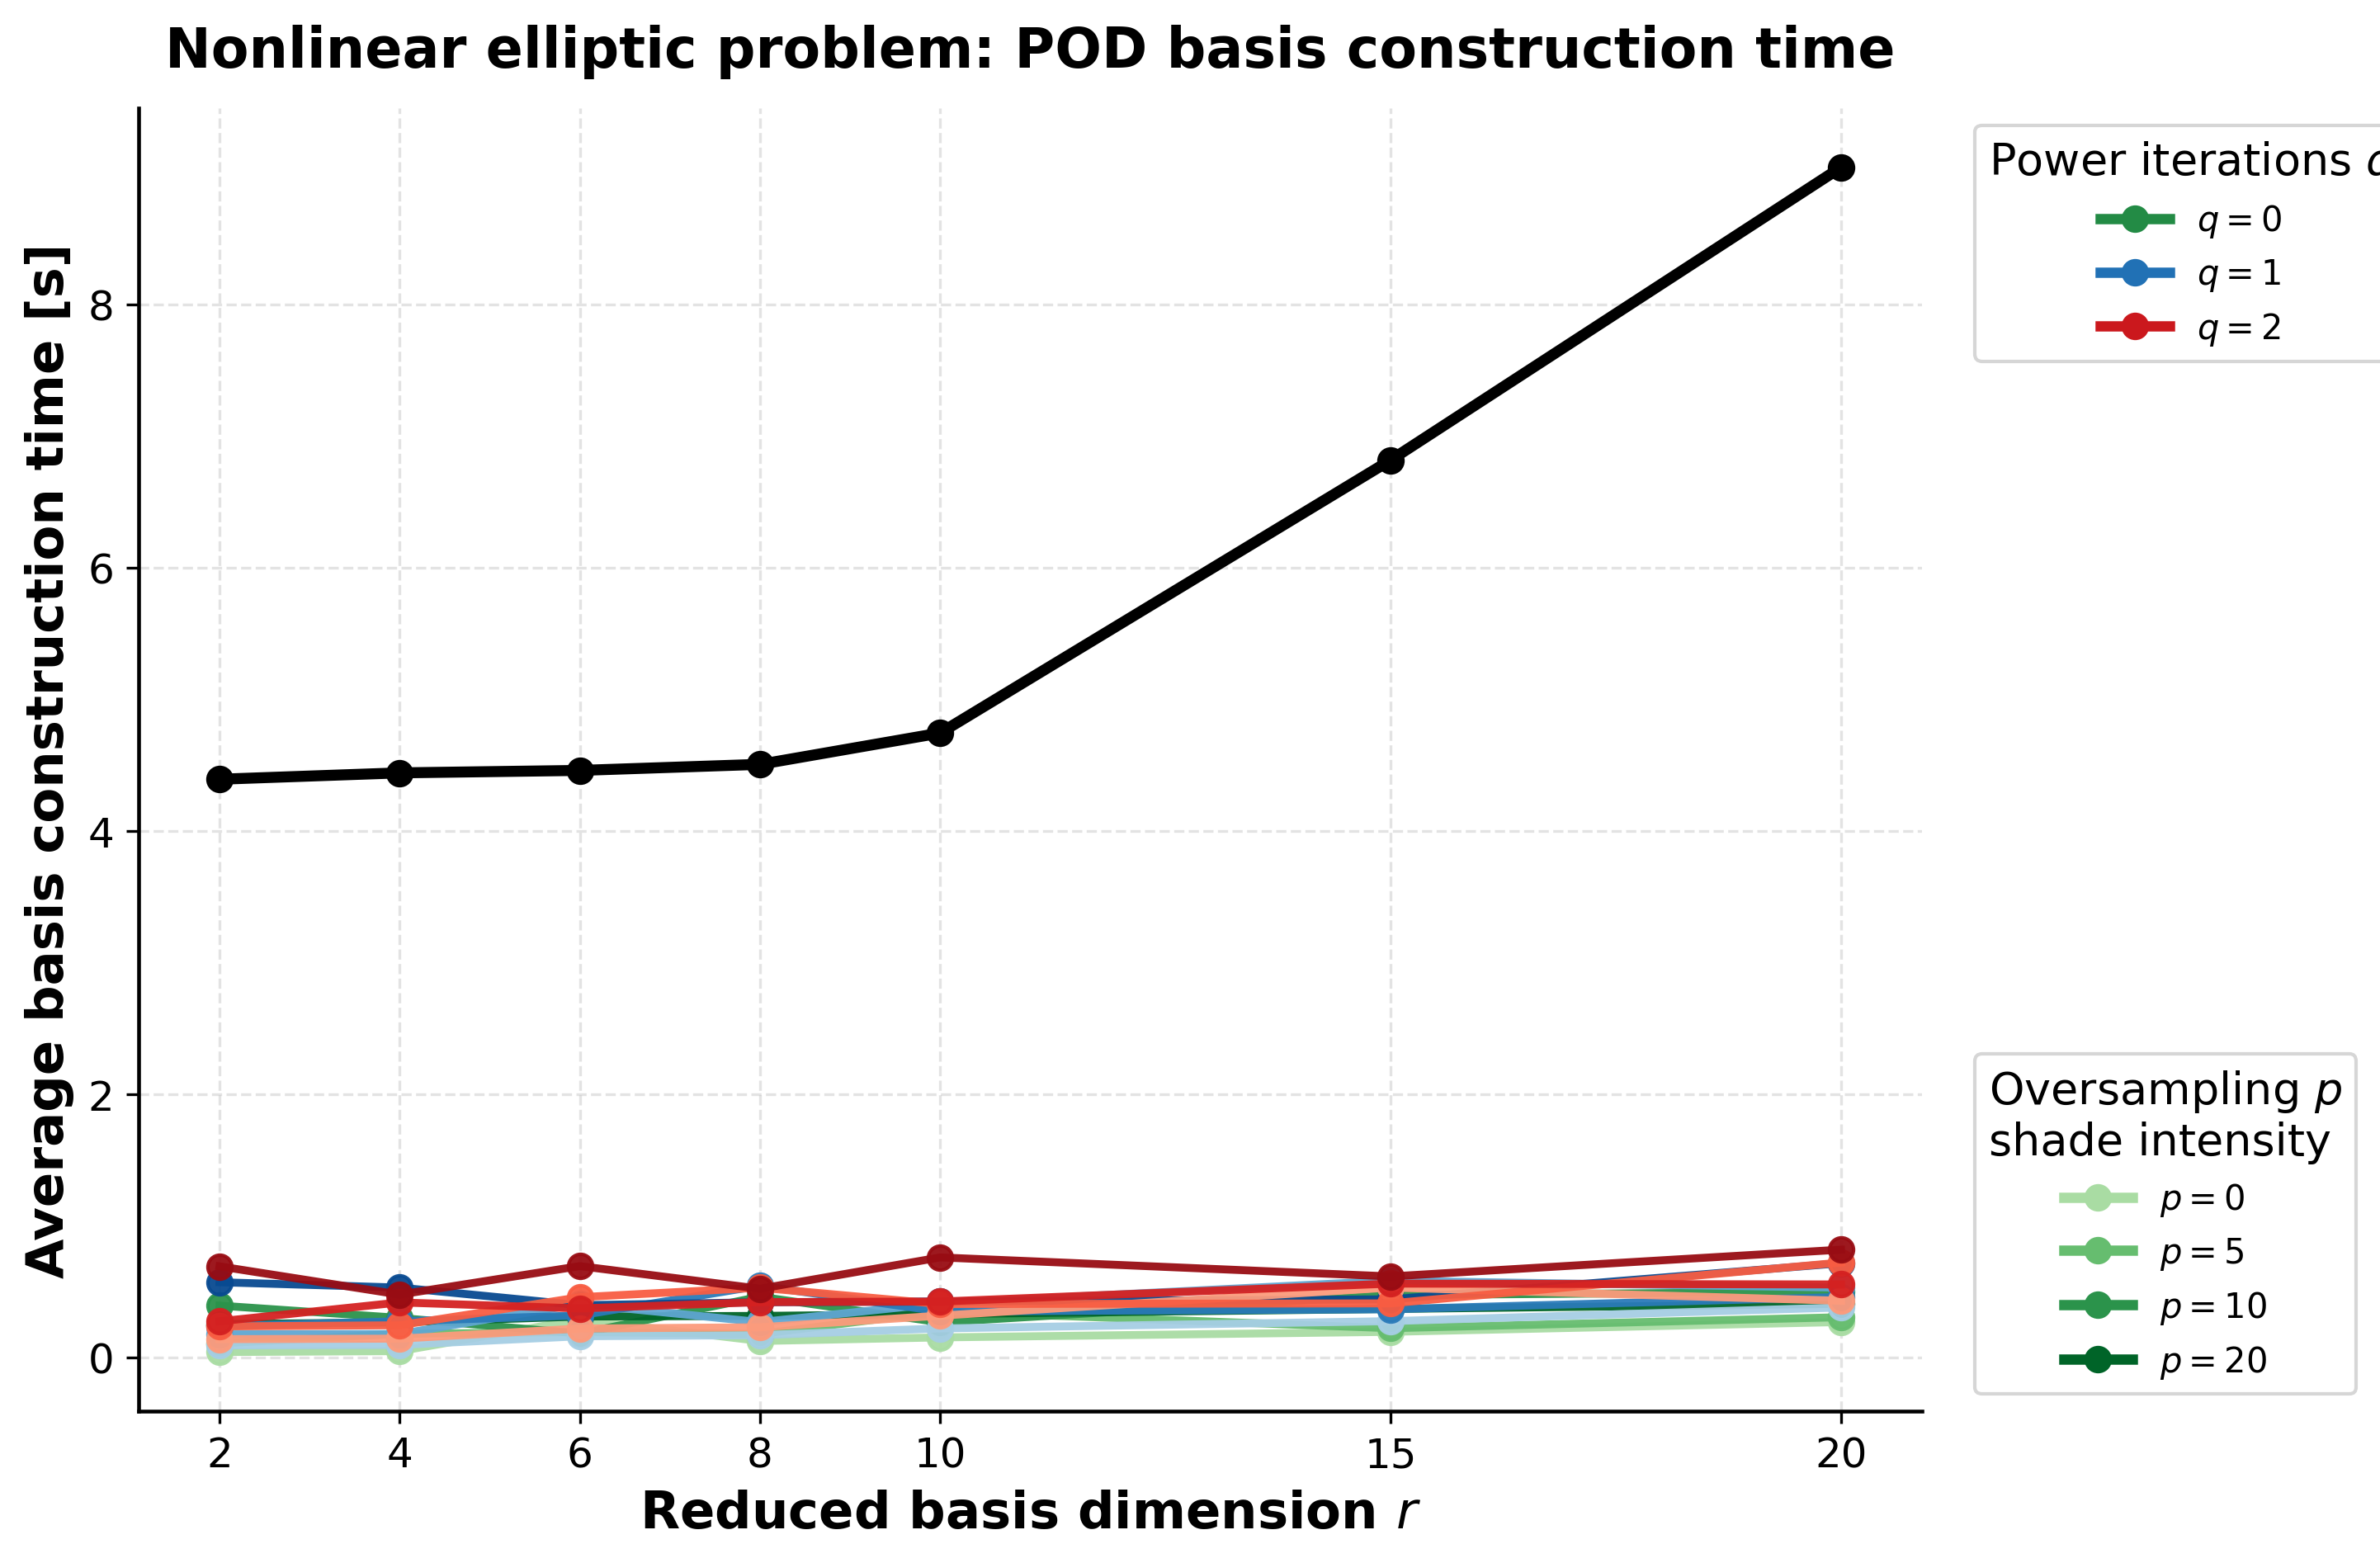
\includegraphics[width=\textwidth,height=0.42\textheight,keepaspectratio]{figures/elliptic_pod_basis_time.png}

\column{0.33\textwidth}
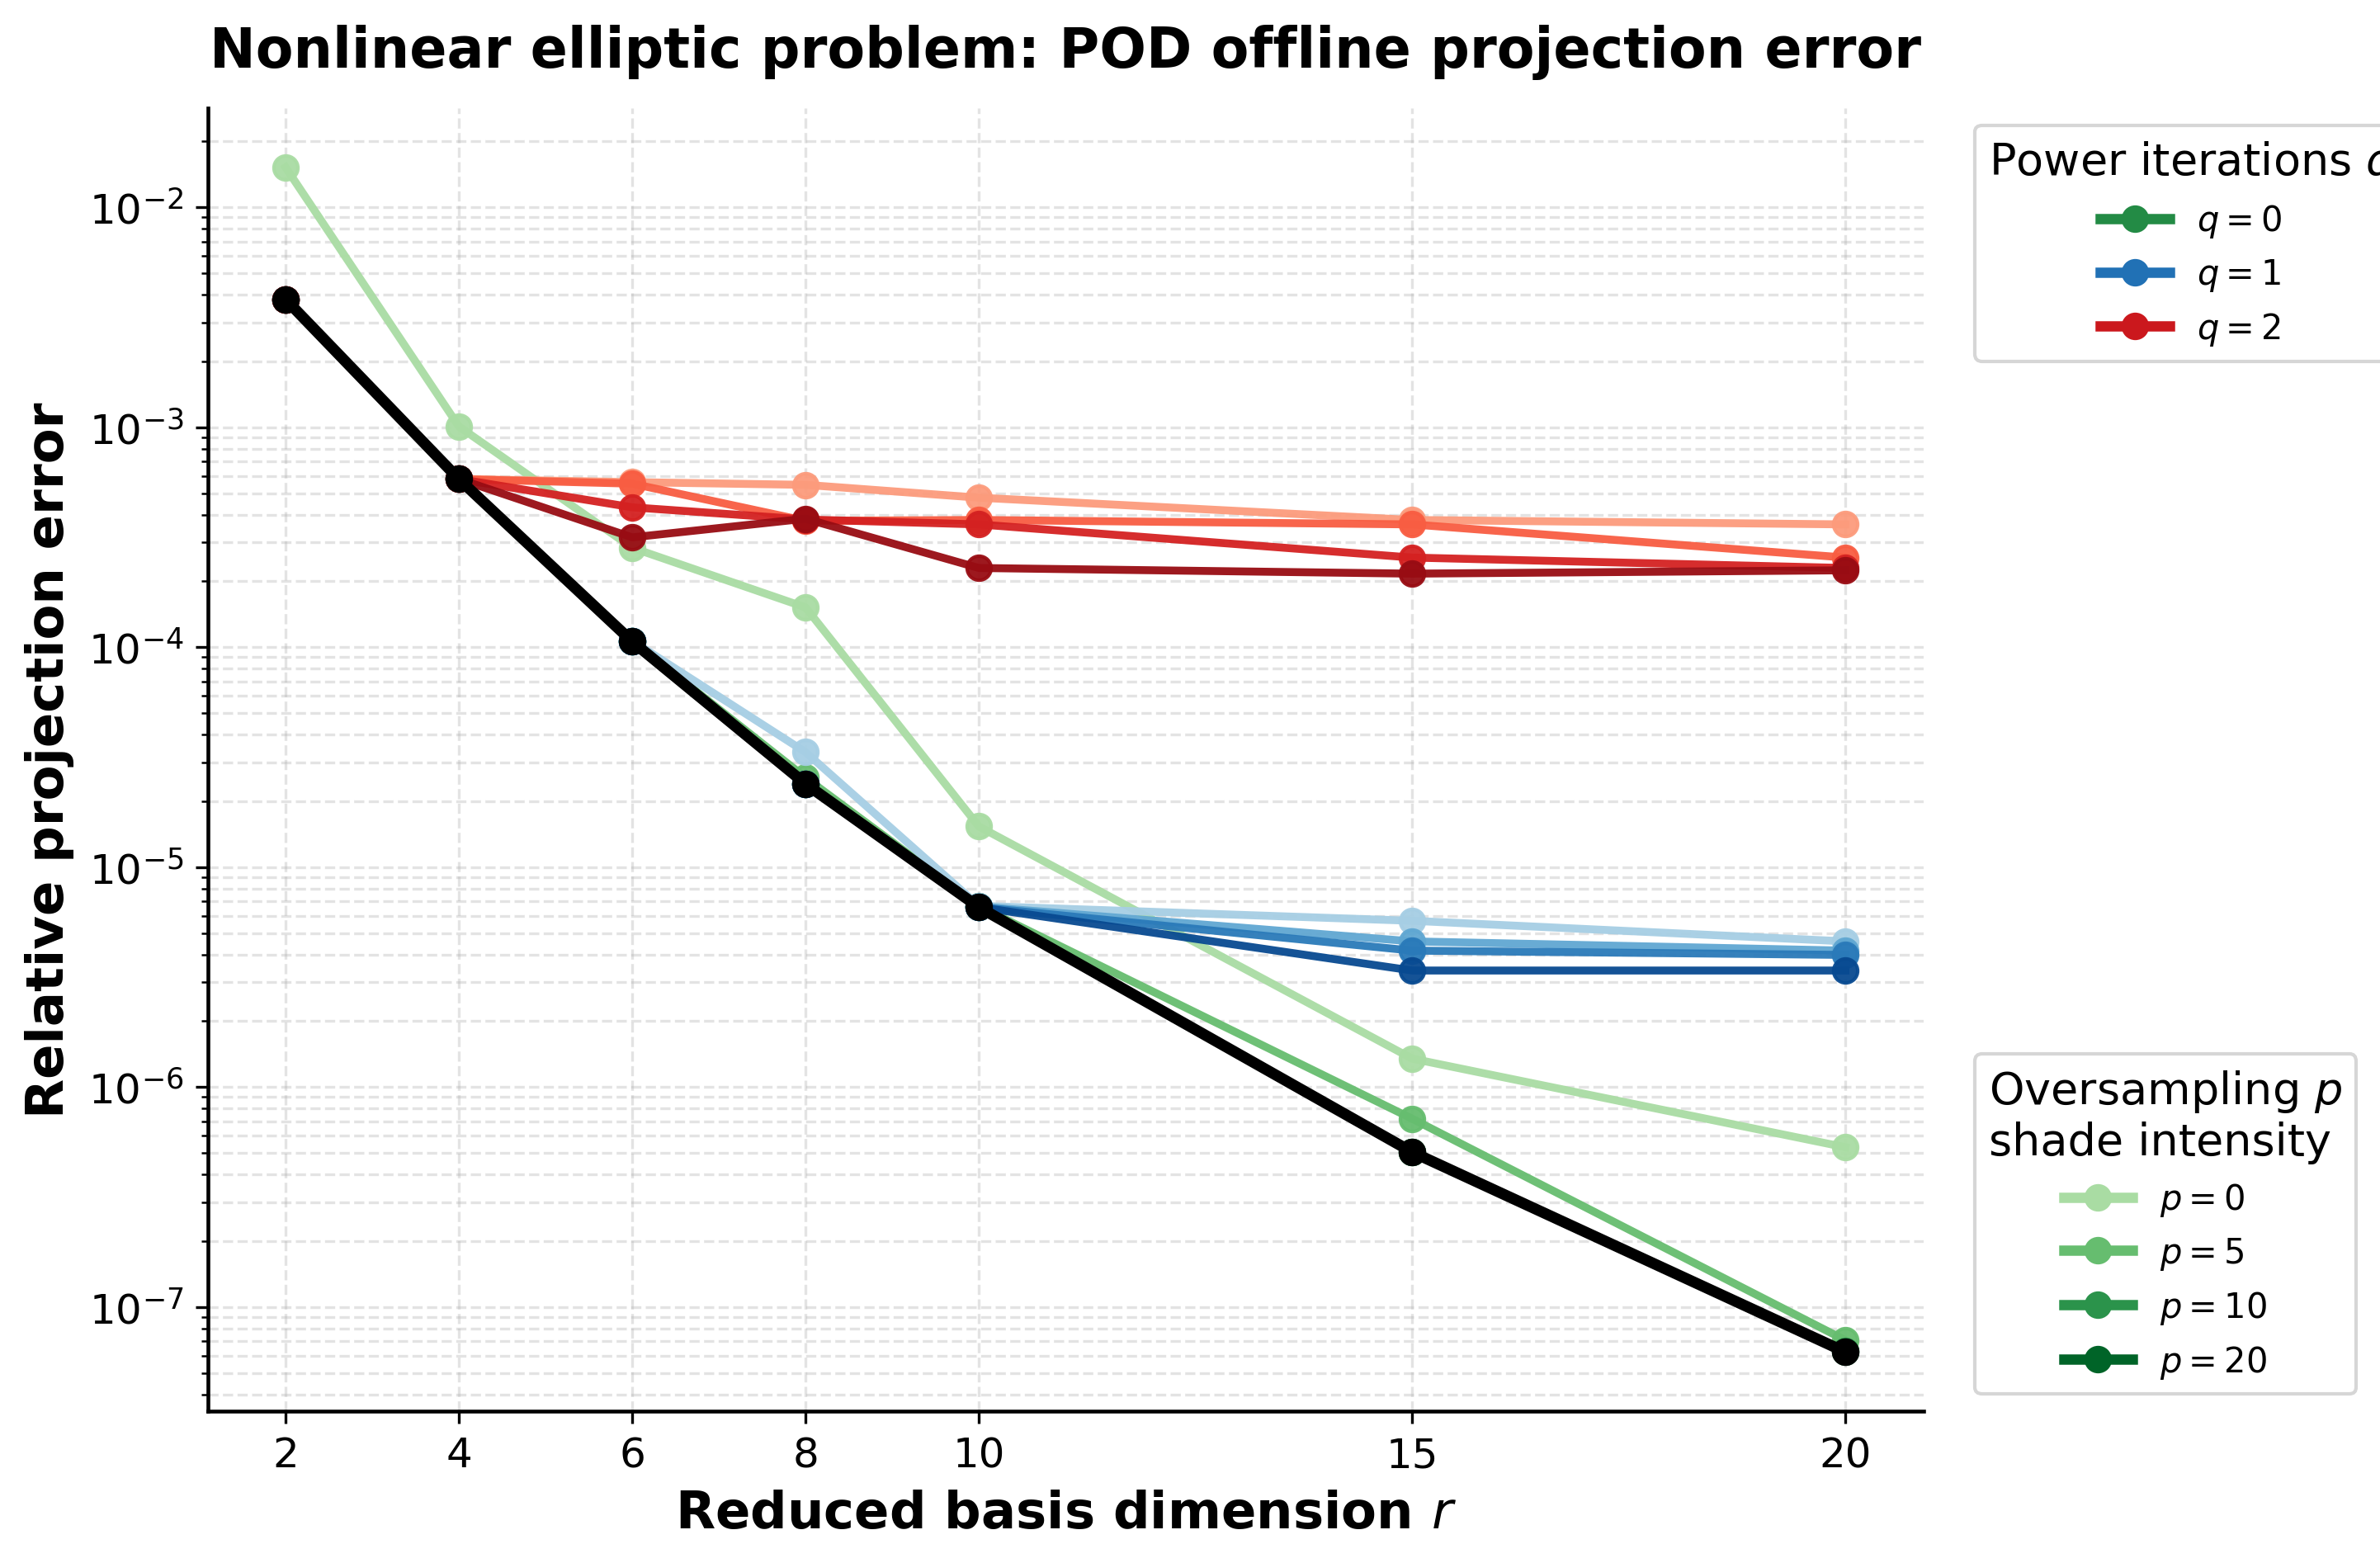
\includegraphics[width=\textwidth,height=0.42\textheight,keepaspectratio]{figures/elliptic_pod_offline_error.png}

\column{0.33\textwidth}
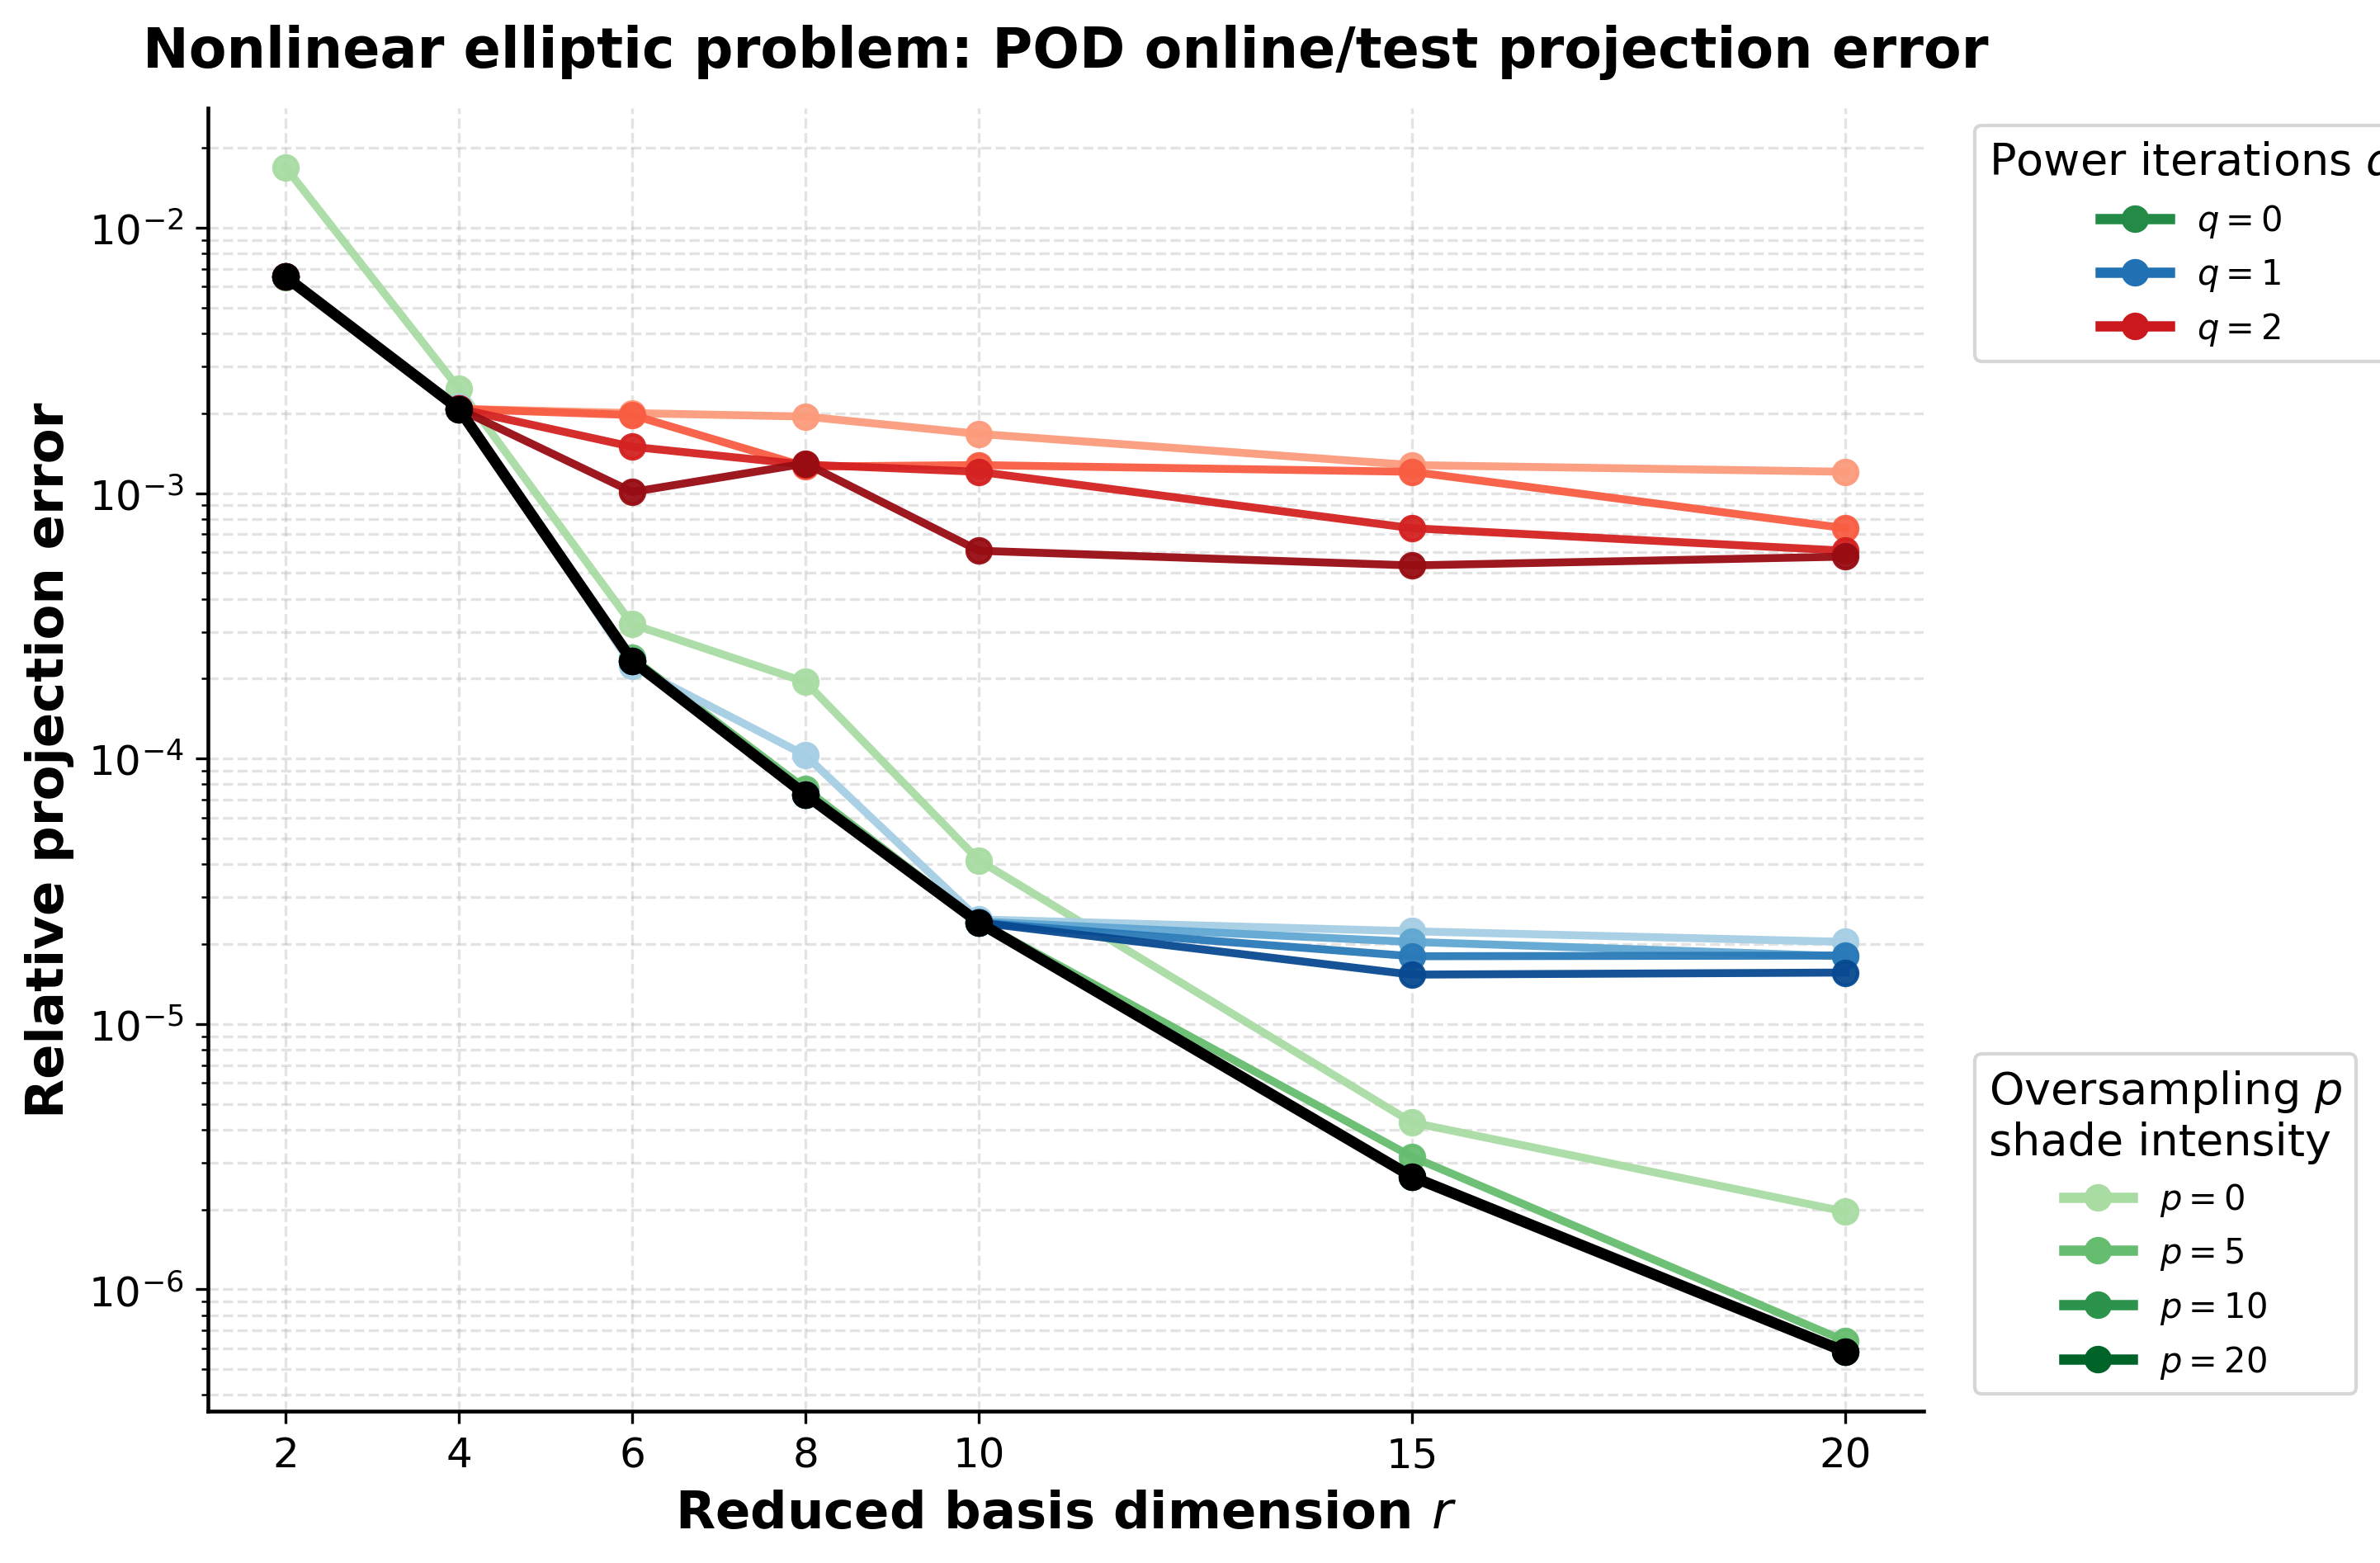
\includegraphics[width=\textwidth,height=0.42\textheight,keepaspectratio]{figures/elliptic_pod_online_error.png}

\end{columns}

\vspace{0.25cm}

\begin{block}{Lettura dei grafici}
\begin{itemize}
  \item La base POD e' costruita solo sui parametri di train.
  \item L'errore offline misura la ricostruzione dei parametri gia' usati.
  \item L'errore online/test misura la ricostruzione sui parametri tenuti fuori dalla base.
\end{itemize}
\end{block}

\end{frame}

% 23
\begin{frame}{PDE ellittica: nonlinear snapshots per DEIM}
Il termine non lineare del problema ellittico e':
\[
s(u;\mu)=\frac{\mu_1}{\mu_2}\left(e^{\mu_2u}-1\right).
\]
Dopo aver risolto il full order problem per ogni parametro $\mu_j$, il notebook costruisce:
\[
\widehat F_{\mathrm{ell}}=
\begin{bmatrix}
s(u(\mu_0);\mu_0)&
s(u(\mu_1);\mu_1)&
\cdots&
s(u(\mu_{255});\mu_{255})
\end{bmatrix}.
\]
\begin{itemize}
  \item La base DEIM $\Phi$ e gli indici $P$ sono calcolati da $\widehat F_{\mathrm{ell,train}}$.
  \item Per il test si usa la funzione non lineare corretta per ogni parametro di test.
  \item L'errore riportato e' la media degli errori relativi sui parametri train o test.
\end{itemize}
\end{frame}

% 24
\begin{frame}{Risultati PDE ellittica: POD-DEIM}
\begin{columns}[T]

\column{0.33\textwidth}
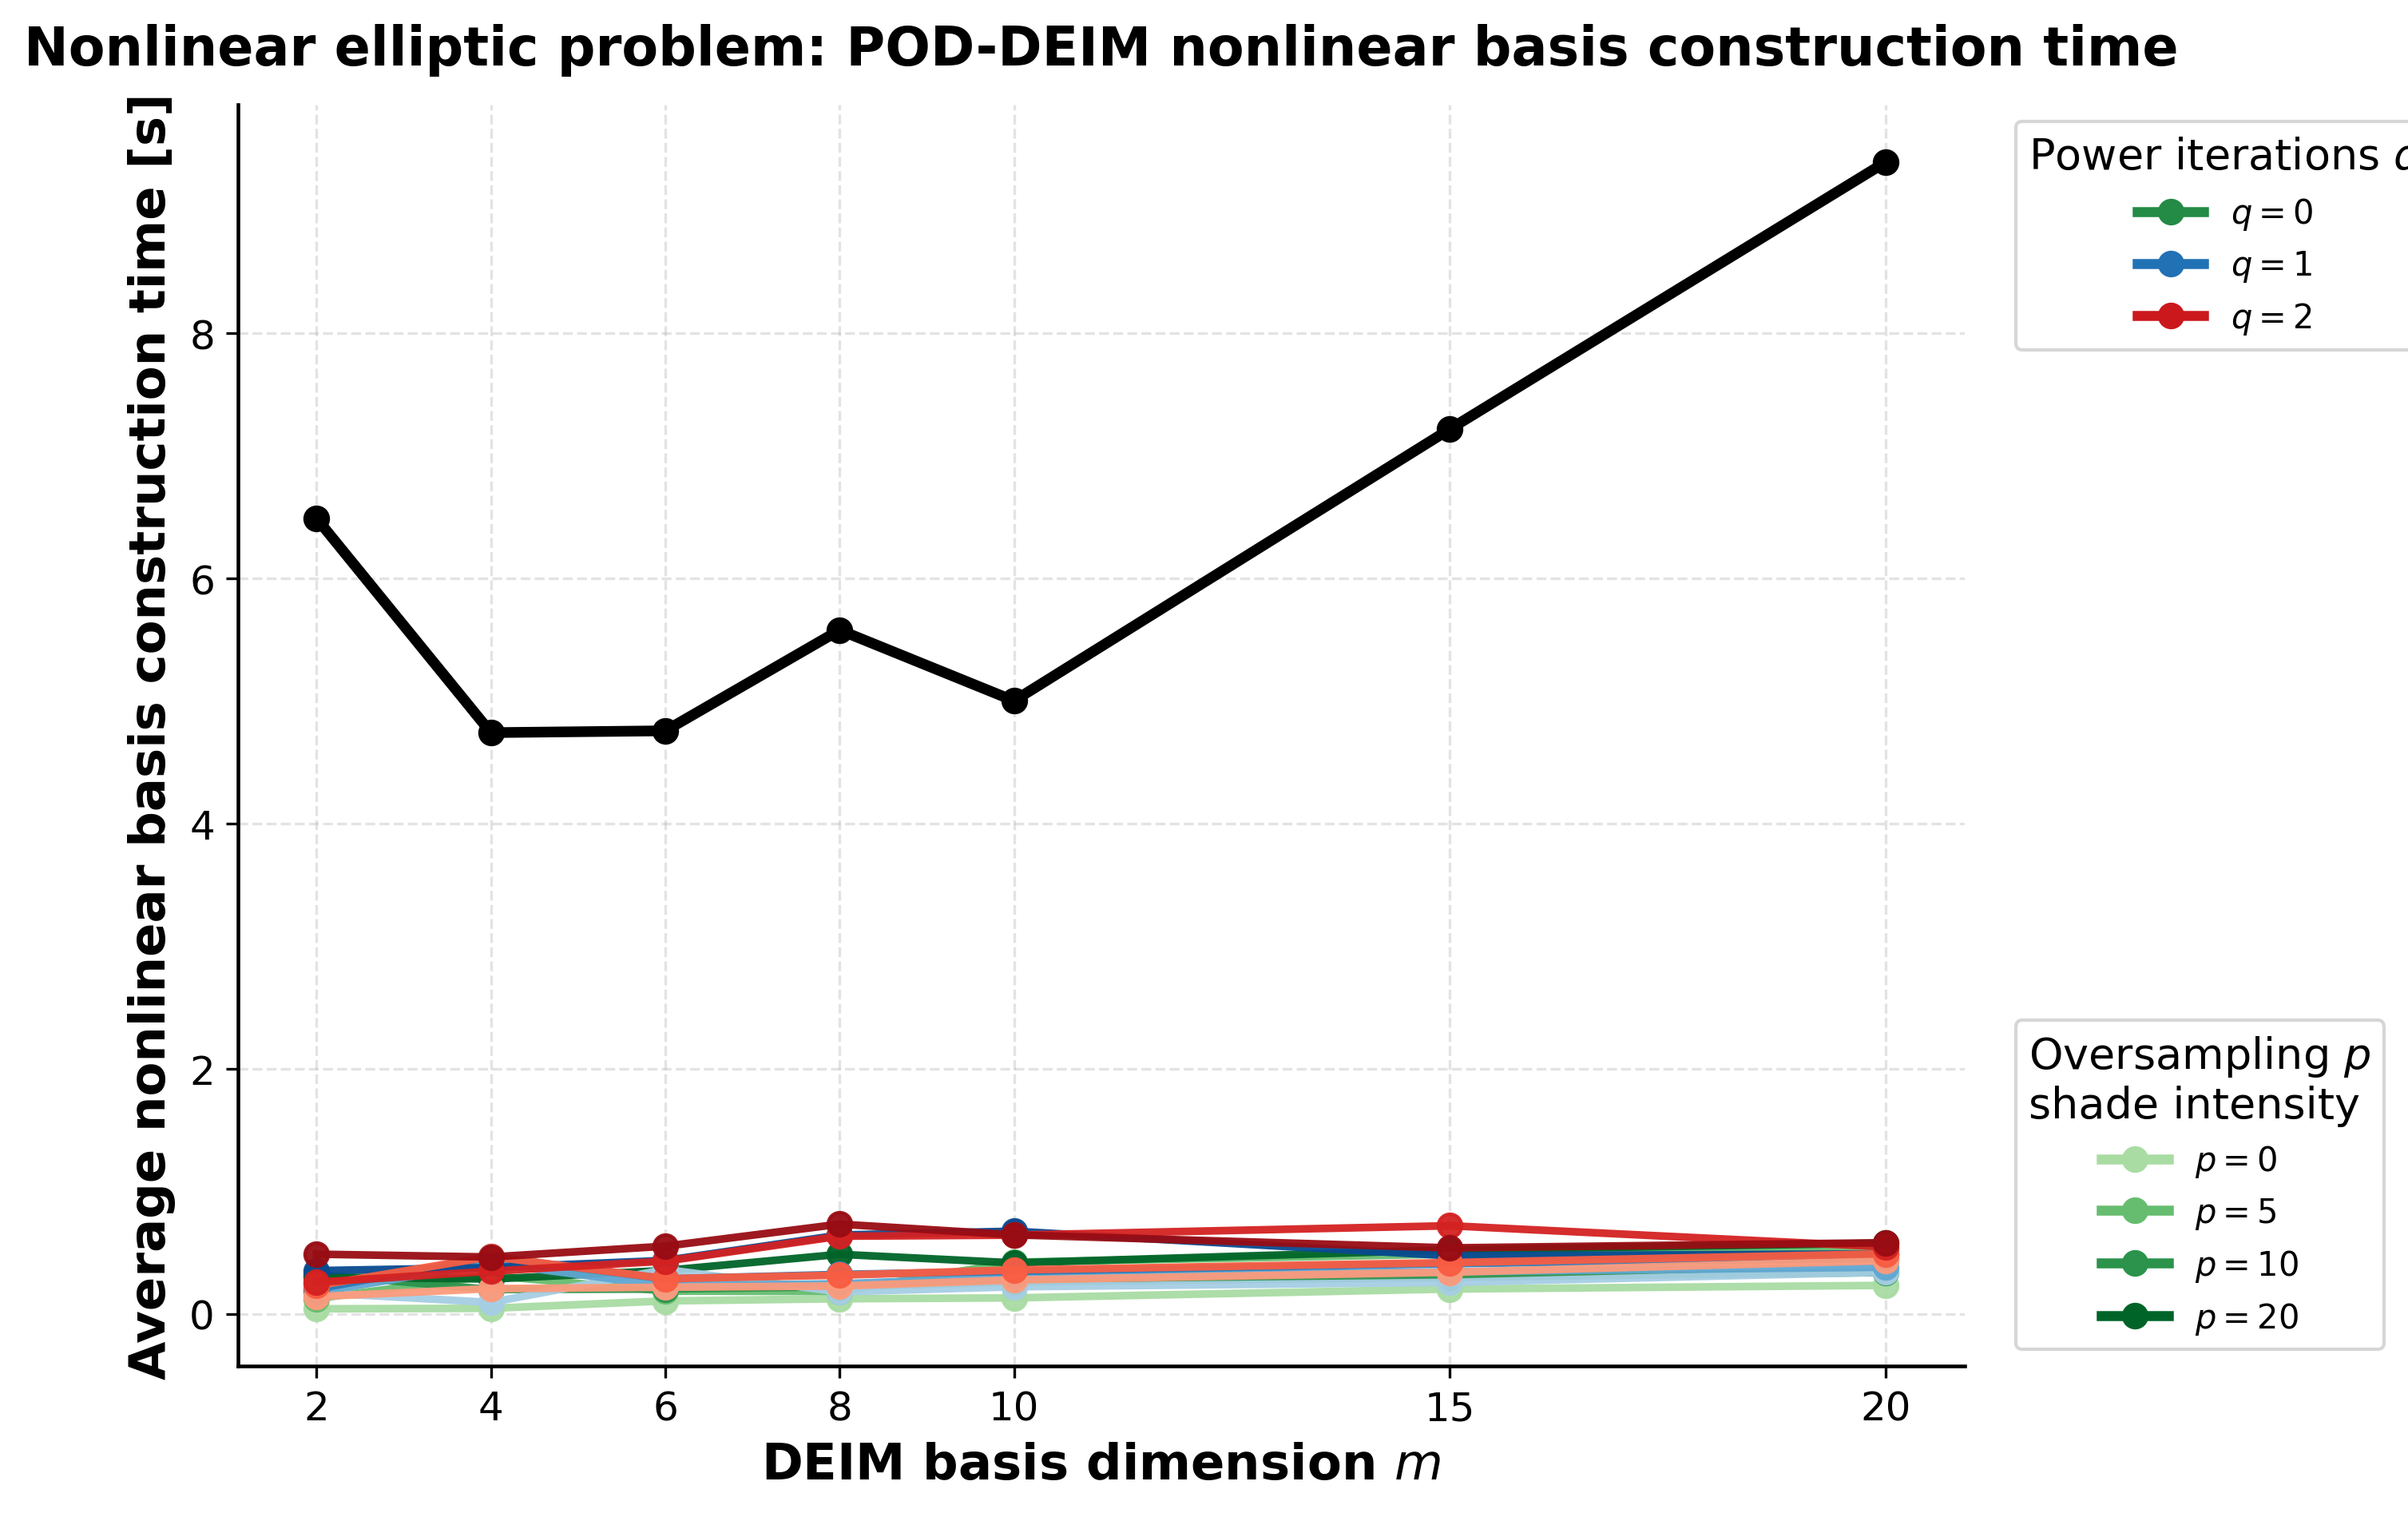
\includegraphics[width=\textwidth,height=0.42\textheight,keepaspectratio]{figures/elliptic_deim_basis_time.png}

\column{0.33\textwidth}
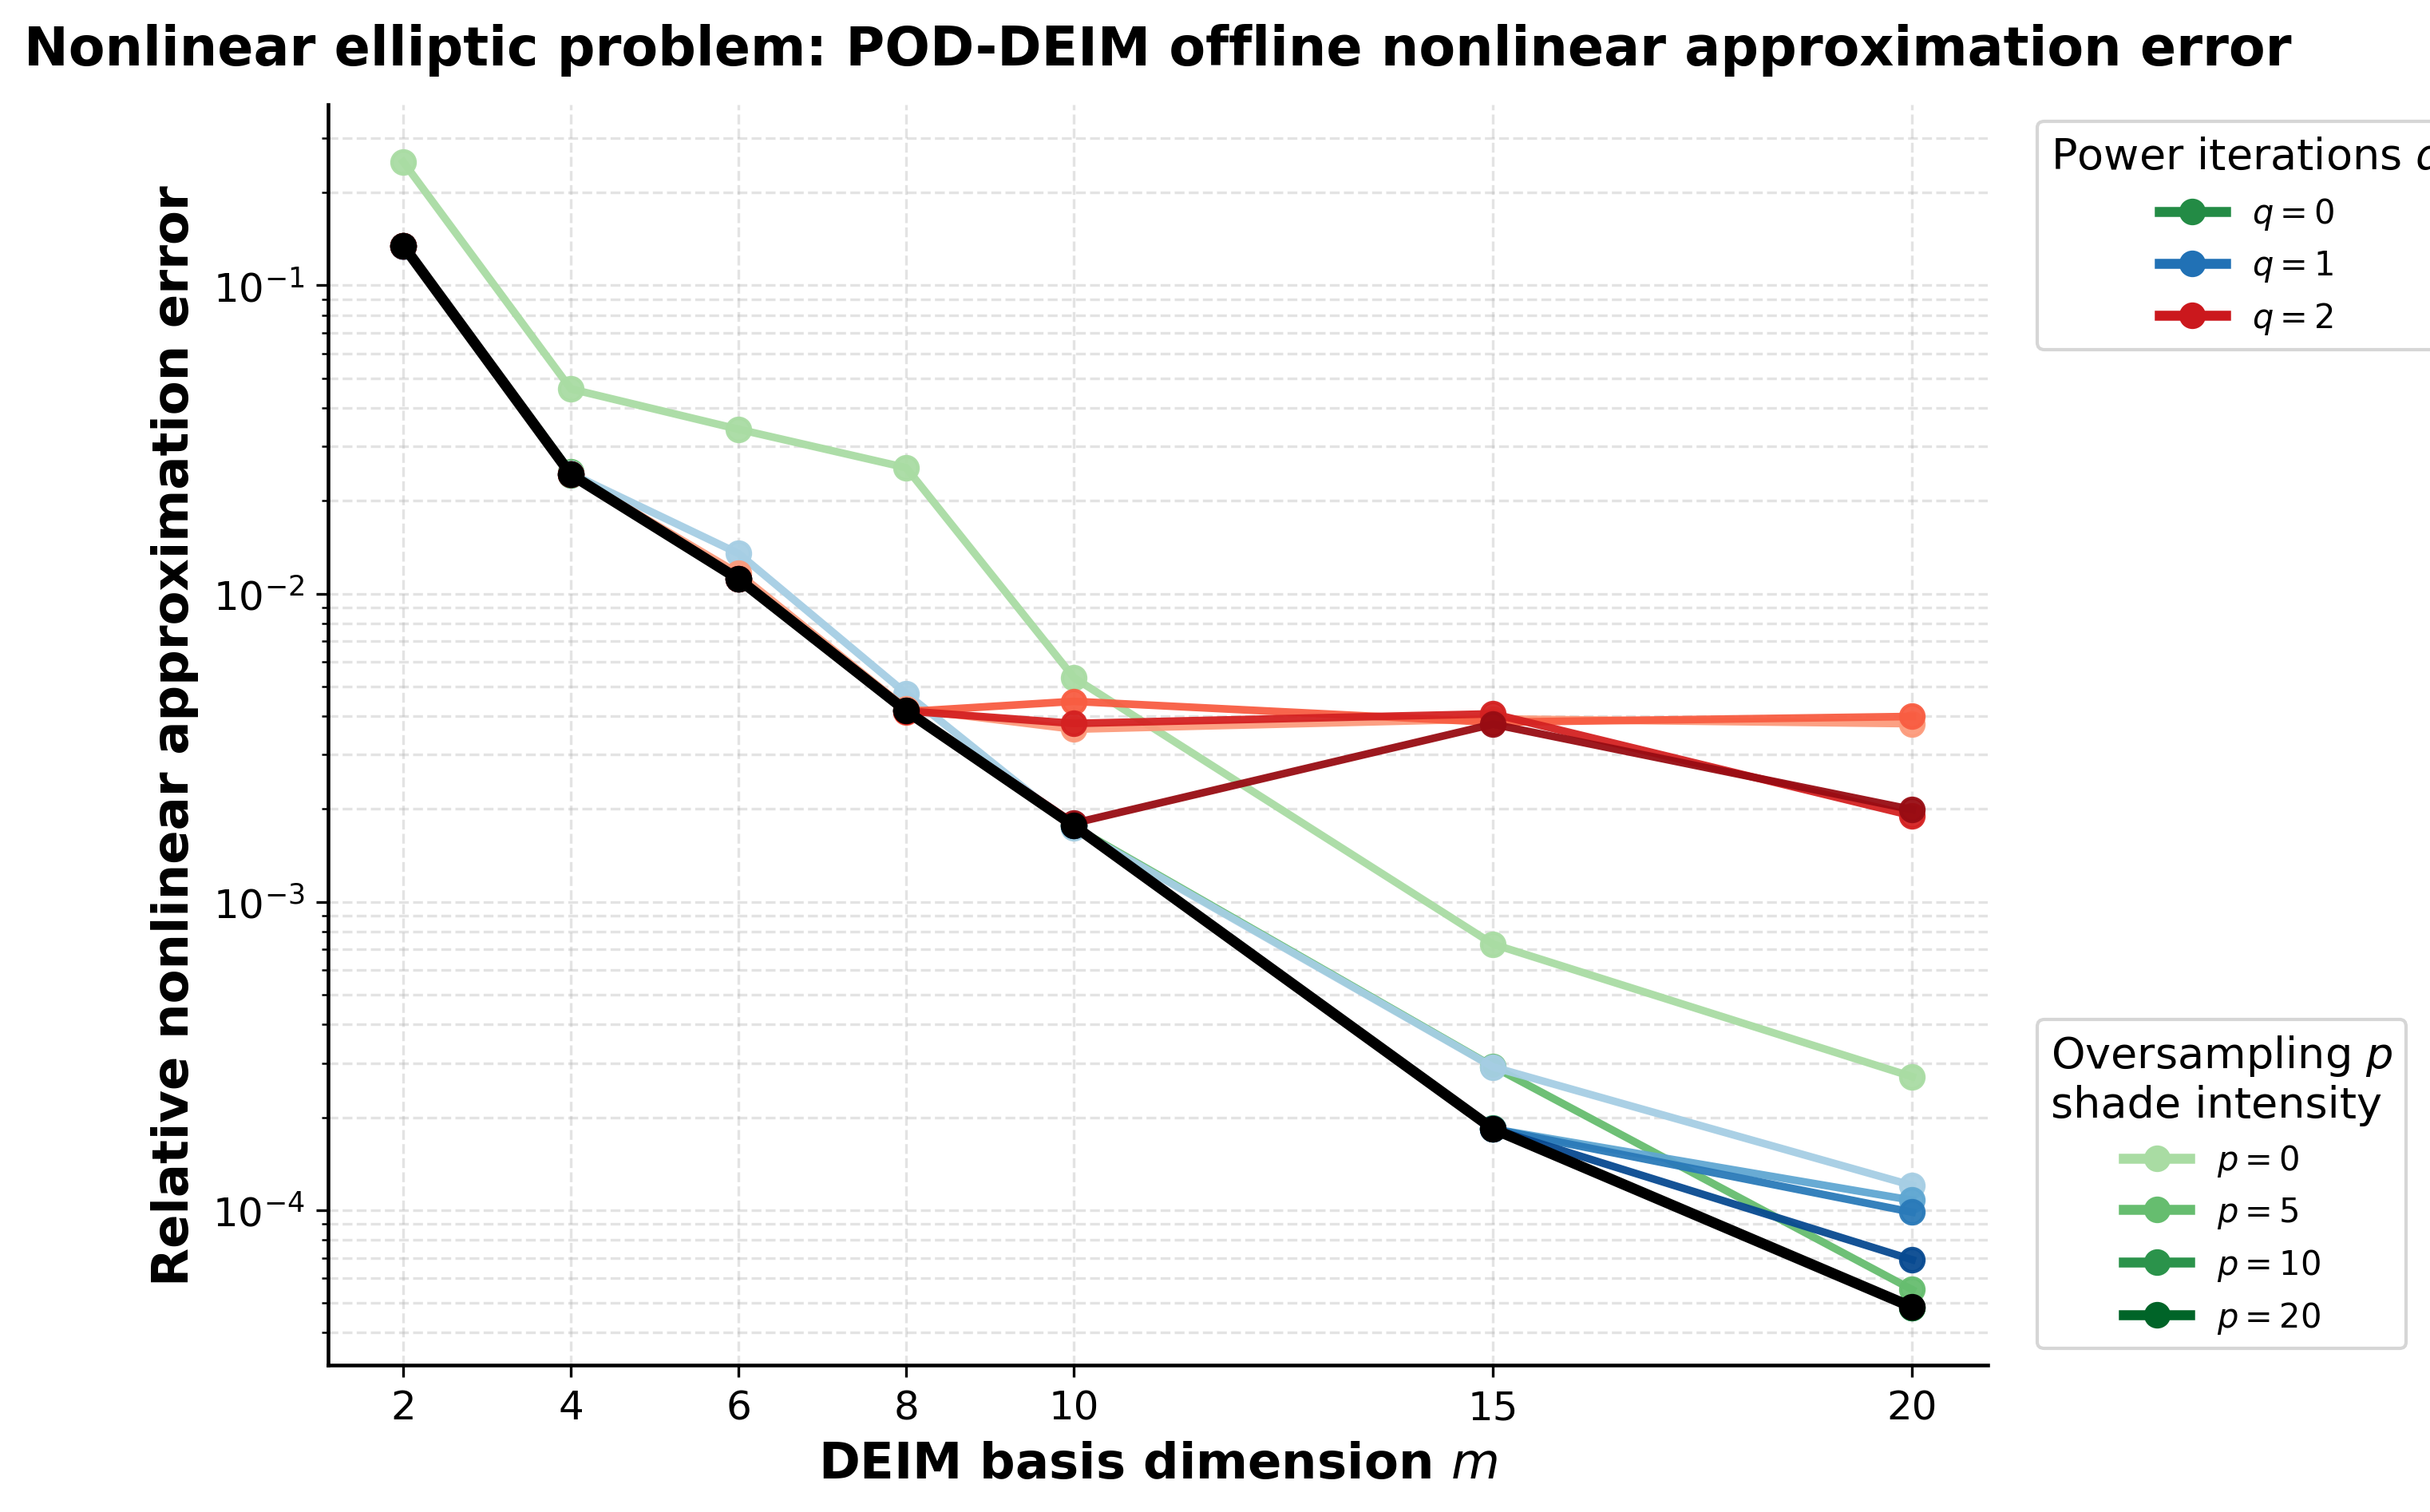
\includegraphics[width=\textwidth,height=0.42\textheight,keepaspectratio]{figures/elliptic_deim_offline_error.png}

\column{0.33\textwidth}
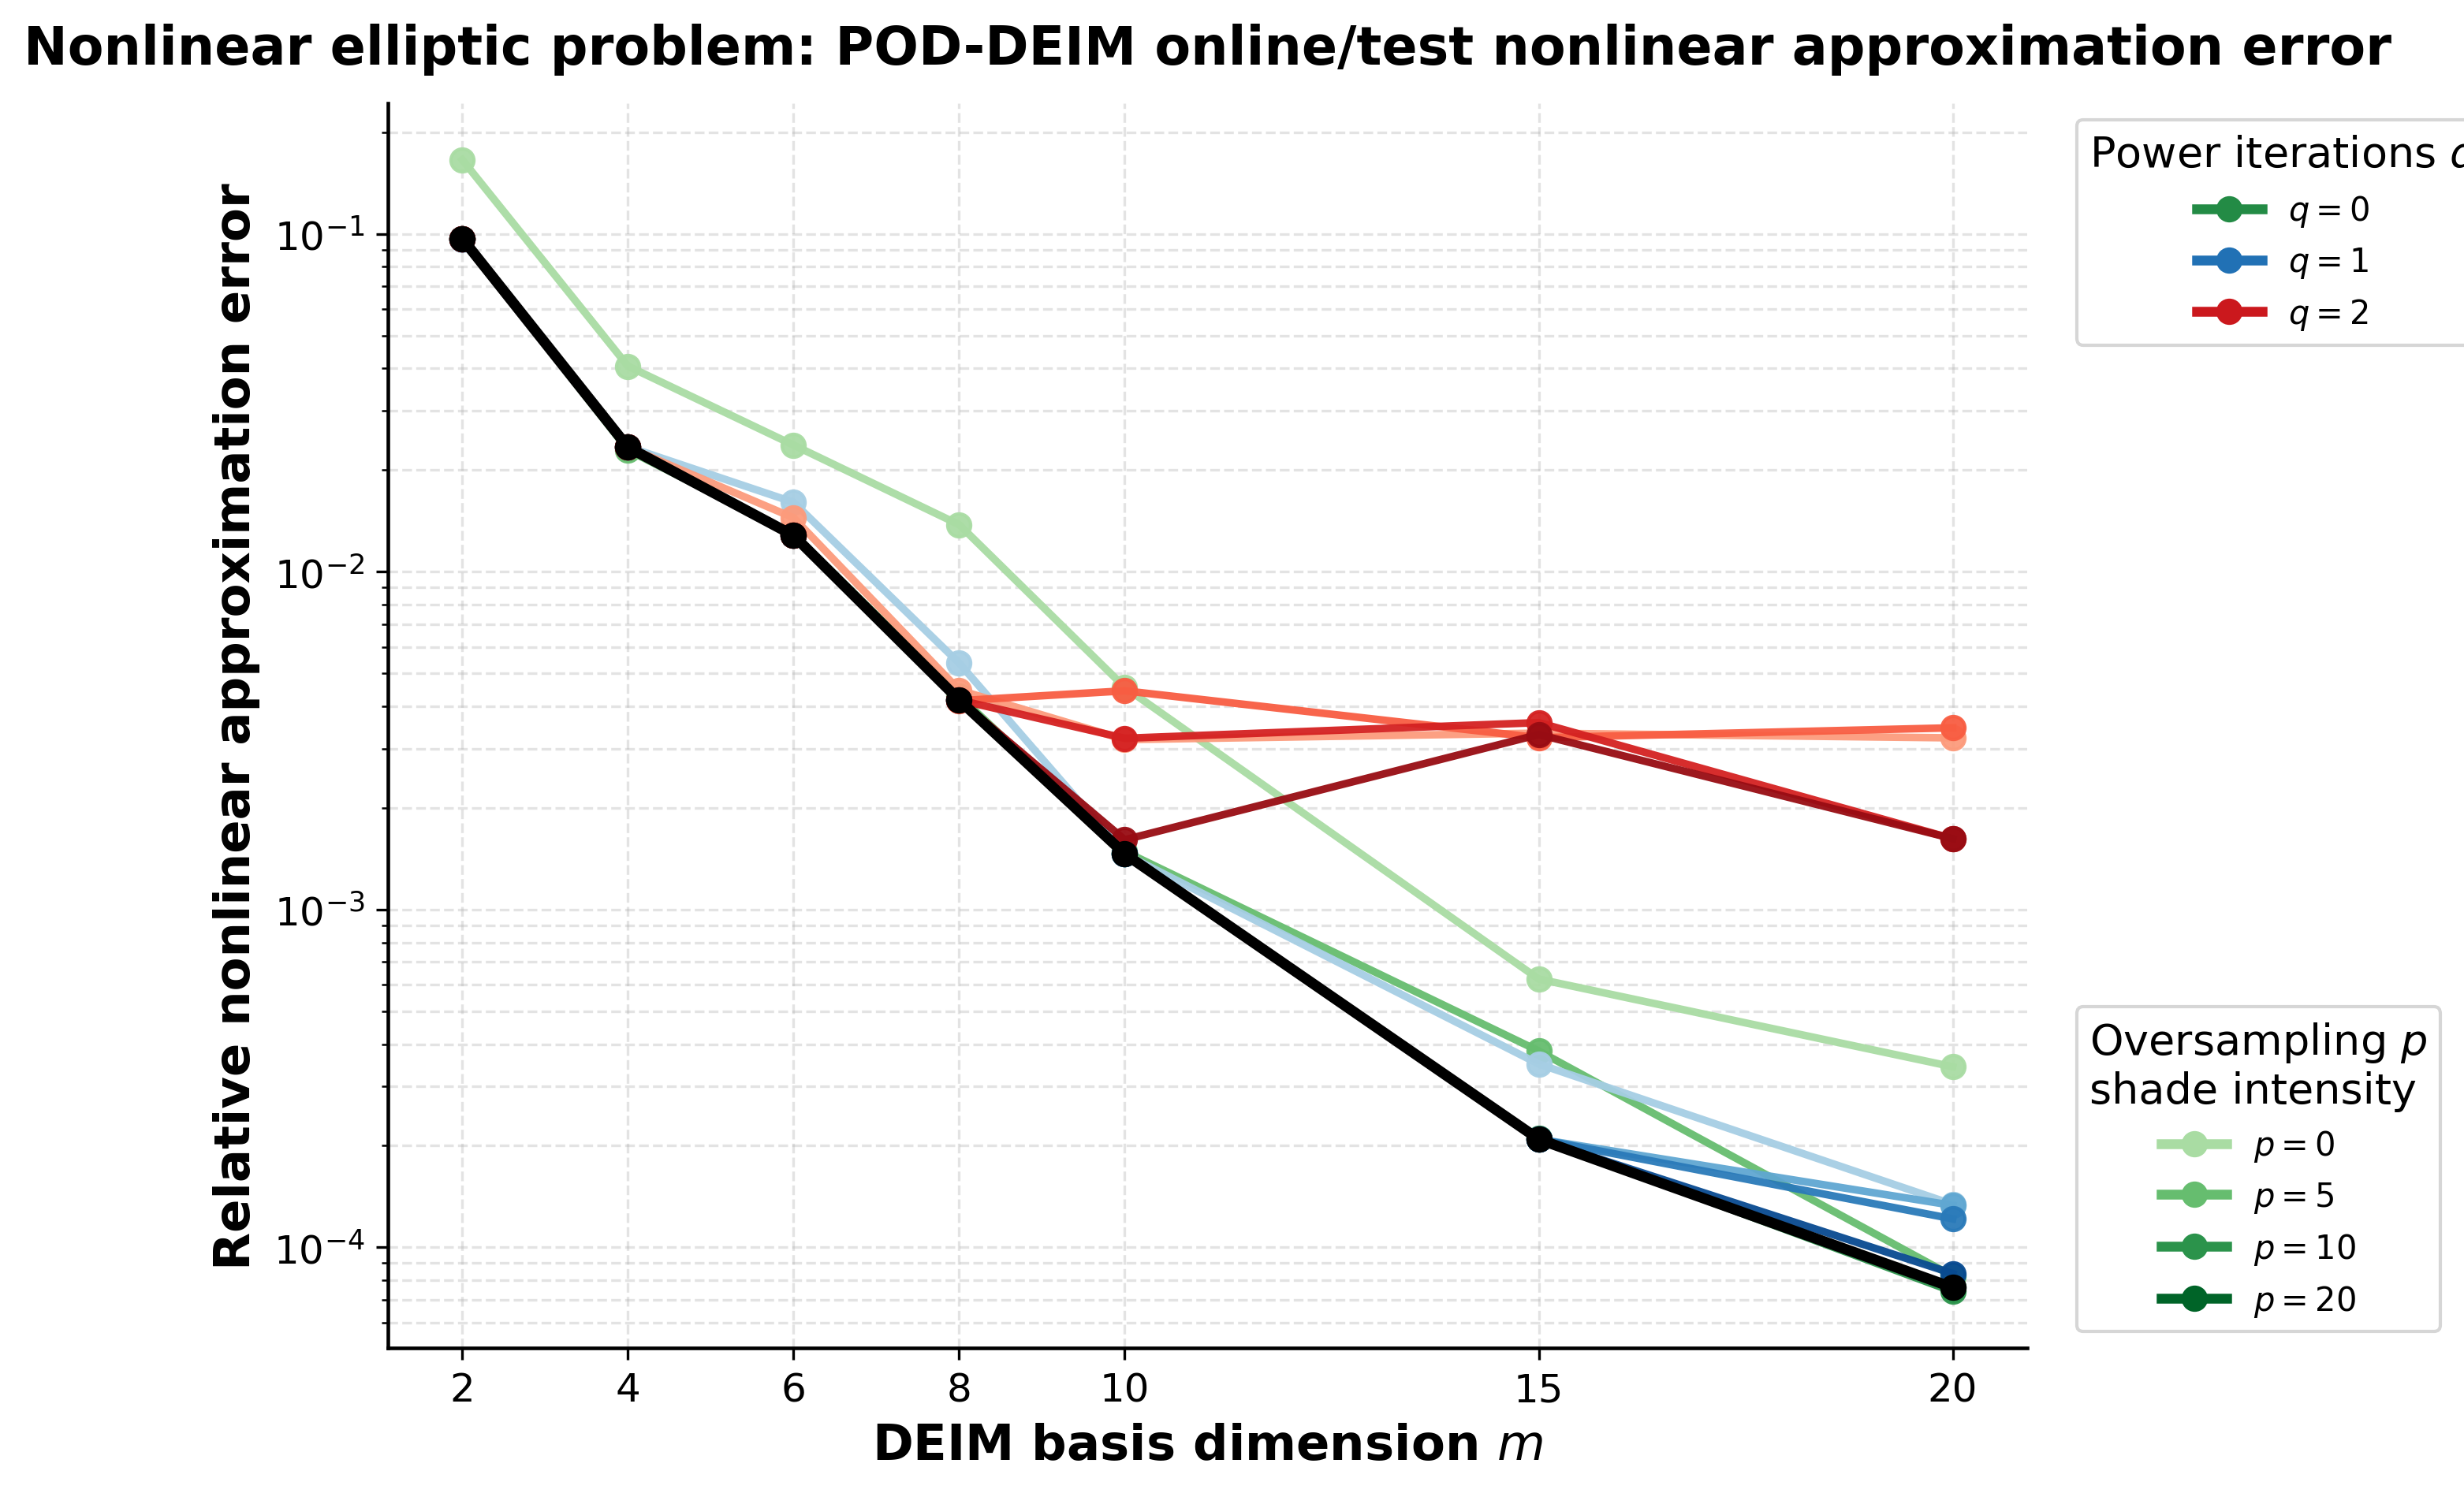
\includegraphics[width=\textwidth,height=0.42\textheight,keepaspectratio]{figures/elliptic_deim_online_error.png}

\end{columns}

\vspace{0.25cm}

\begin{block}{Lettura dei grafici}
\begin{itemize}
  \item La base non lineare e' costruita sui nonlinear snapshots di train.
  \item L'errore test controlla se gli indici DEIM scelti generalizzano a nuovi parametri.
  \item Il confronto SVD/rSVD riguarda il tempo di costruzione della base e l'accuratezza finale.
\end{itemize}
\end{block}

\end{frame}

% 25
\begin{frame}{Conclusioni e considerazioni}
\begin{itemize}
  \item La rSVD approssima la SVD troncata con buona accuratezza e costo computazionale inferiore.
  \item L'oversampling $p$ è un parametro semplice ma molto efficace per stabilizzare l'approssimazione.
  \item Le power iterations $q$ non vanno usate automaticamente: possono aiutare con spettri lenti, ma in alcuni test hanno peggiorato l'errore.
  \item Nelle immagini, rSVD ottiene ricostruzioni simili alla SVD con tempi minori. (q=1 meglio di q=0)
  \item Nei ROM per PDE, rSVD accelera la fase offline; DEIM riduce il costo online dei termini non lineari (q=0 meglio di q=1 e q=2).
\end{itemize}
\end{frame}

% 20
\begin{frame}{Riferimenti}
\small
\begin{thebibliography}{9}
\bibitem{halko2011}
N. Halko, P. G. Martinsson, J. A. Tropp, \emph{Finding Structure with Randomness: Probabilistic Algorithms for Constructing Approximate Matrix Decompositions}, SIAM Review, 2011.
\bibitem{deim2010}
S. Chaturantabut, D. C. Sorensen, \emph{Nonlinear Model Reduction via Discrete Empirical Interpolation}, SIAM Journal on Scientific Computing, 2010.
\bibitem{golub2013}
G. H. Golub, C. F. Van Loan, \emph{Matrix Computations}, Johns Hopkins University Press, 2013.
\bibitem{quarteroni2015}
A. Quarteroni, A. Manzoni, F. Negri, \emph{Reduced Basis Methods for Partial Differential Equations}, Springer, 2015.
\end{thebibliography}
\end{frame}

\end{document}

